\chapter{Modelling Lubricated Bearings in a Flexible Multi-Body Dynamic Environment}
\label{Lubricated FMBD}

\section{Introduction}
The previous chapter highlights the necessity of implicitly modelling the EHL film at the roller-race contact. A workflow was established to implicitly account for the lubricant film at the roller-race conjunction. However, bearing motion is obtained experimentally, which limits the investigation to component level analysis. Since this work aims to investigate the effect of the EHL film at system level, and dynamic model must be developed.

This chapter presents a new flexible dynamic model for drive systems comprising lubricated bearings operating under conditions representative of electrified vehicle powertrains. This is achieved by embedding a non-linear lubricated bearing model within an FMBD model; something which has not, to the authors’ knowledge, been reported on hitherto. The time-varying system operating conditions reflect that of an electrified powertrain. The kinematic behaviour of a flexible shaft at each time step of a dynamic simulation is passed to the bearing model. A contact slicing method \cite{Andreason1973} is employed to calculate the reaction forces of the individual rolling elements based on the roller–race contact deflection \cite{Lundberg1949}. The total deflection is influenced by the thickness of the EHL film within the contact, which is implicitly included within the analysis through an iterative procedure. The resulting race forces are returned to the system level model and the equations of motion are solved at each time step. Comparisons are made between modelling the bearings as dry and lubricated. The dynamic results including acceleration, force magnitudes and stiffness variations have been obtained for realistic loading conditions of a 54~$kW$ electric hub motor up to speeds of 21~000~$rpm$.

The elastohydrodynamic (EHL) film is shown to increase contact deflection, leading to increased contact forces and total bearing stiffness as rotational speeds increase. Results show that at 21~000~$rpm$, the input bearing EHL film reaches a thickness of 4.15~$\mu m$. The lubricant entrainment increases the roller–race contact deflection, causing the contact stiffness to increase non-linearly with speed. The contribution of the lubricant film leads to a 16.6\% greater bearing stiffness at 21~000~$rpm$ when compared to conventional dry bearing modelling methods used in current multi-body dynamic software.

\section{Methodology}

A co-simulation methodology combines a system level model of a flexible shaft and rigid housing, developed in AVL EXCITE\textsuperscript{TM}, with component level models of the lubricated bearings, developed in MATLAB and Simulink. Operating conditions such as rotational speed and external forces are defined in the system level model. Time step, iteration accuracy and simulation length are also defined. Material, geometric and rheological properties of the bearings are defined in the component level model. The kinematic conditions from the system level model (i.e., displacements and velocities in all active degrees of freedom) are passed to the component level model at each time step. For each individual rolling element, the non-linear force–deflection relationship is employed in conjunction with the EHL film calculations to compute the contact reaction force between the roller and race. The resultant force on the inner bearing race due to the contact forces and orbital positions of all elements is then returned to the system level model. The equations of motion are then solved, and the time step is advanced once numerical convergence is achieved. A flowchart of these models representing each time step of the simulation is shown in Figure \ref{Flowchart of models}.

\begin{figure}
	\centering
	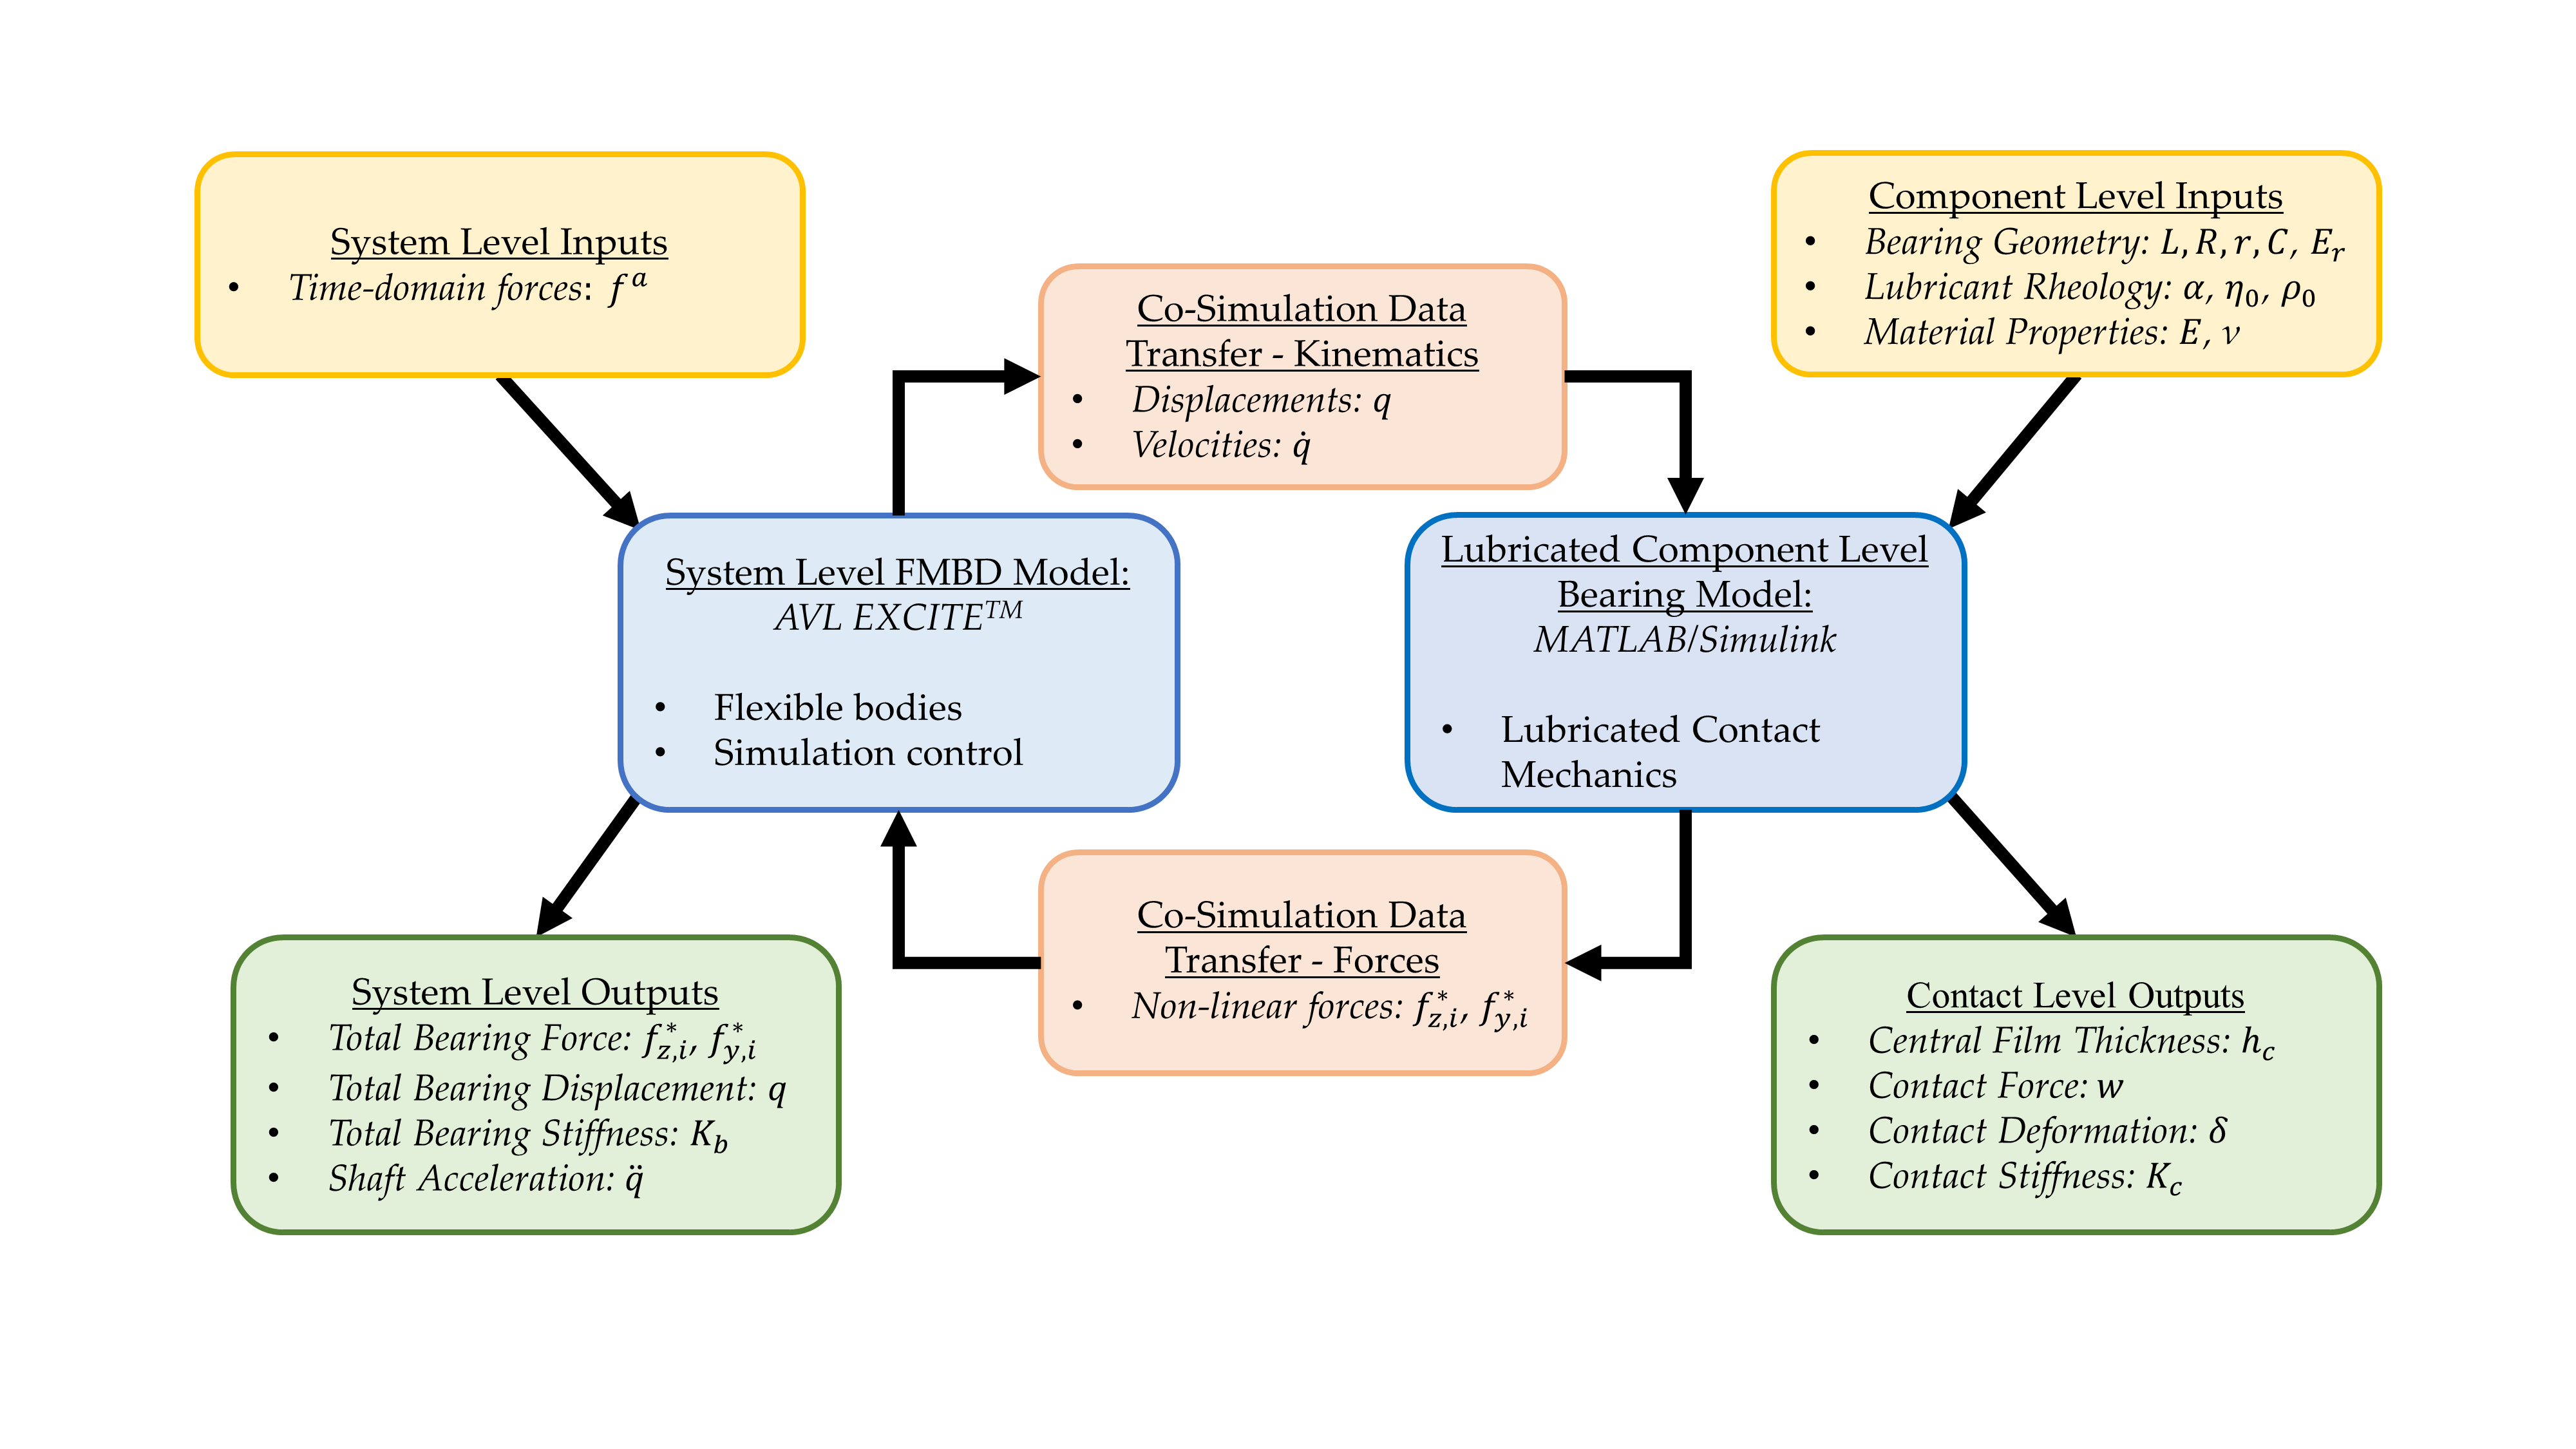
\includegraphics[width=150mm]{FlexiTribo Figure 1. Flowchart of Models.png}
	\caption{Flowchart of models.}
	\label{Flowchart of models}
\end{figure} 

\section{System Level Flexible Model} \label{System level flexible model}

The system level model consists of a flexible shaft, supported by two cylindrical roller bearings in a rigid housing (see Figure \ref{System level model schematic}). The shaft is 472.5~$mm$ between bearing centres, with a 50~$mm$ main diameter and 25~$mm$ diameter bearing seats. The cylindrical roller bearings act as interference elements between the shaft and housing. The shaft can exhibit lateral motion in both vertical ($z$) and horizontal ($y$) directions and rotation about the $x$-axis (see Figure \ref{System level model schematic}). External load is applied at the shaft centre as a time-varying input force, to simulate the gear mesh excitation, or as a static load. The rotational speed is input as a boundary condition.

\begin{figure}
	\centering  
	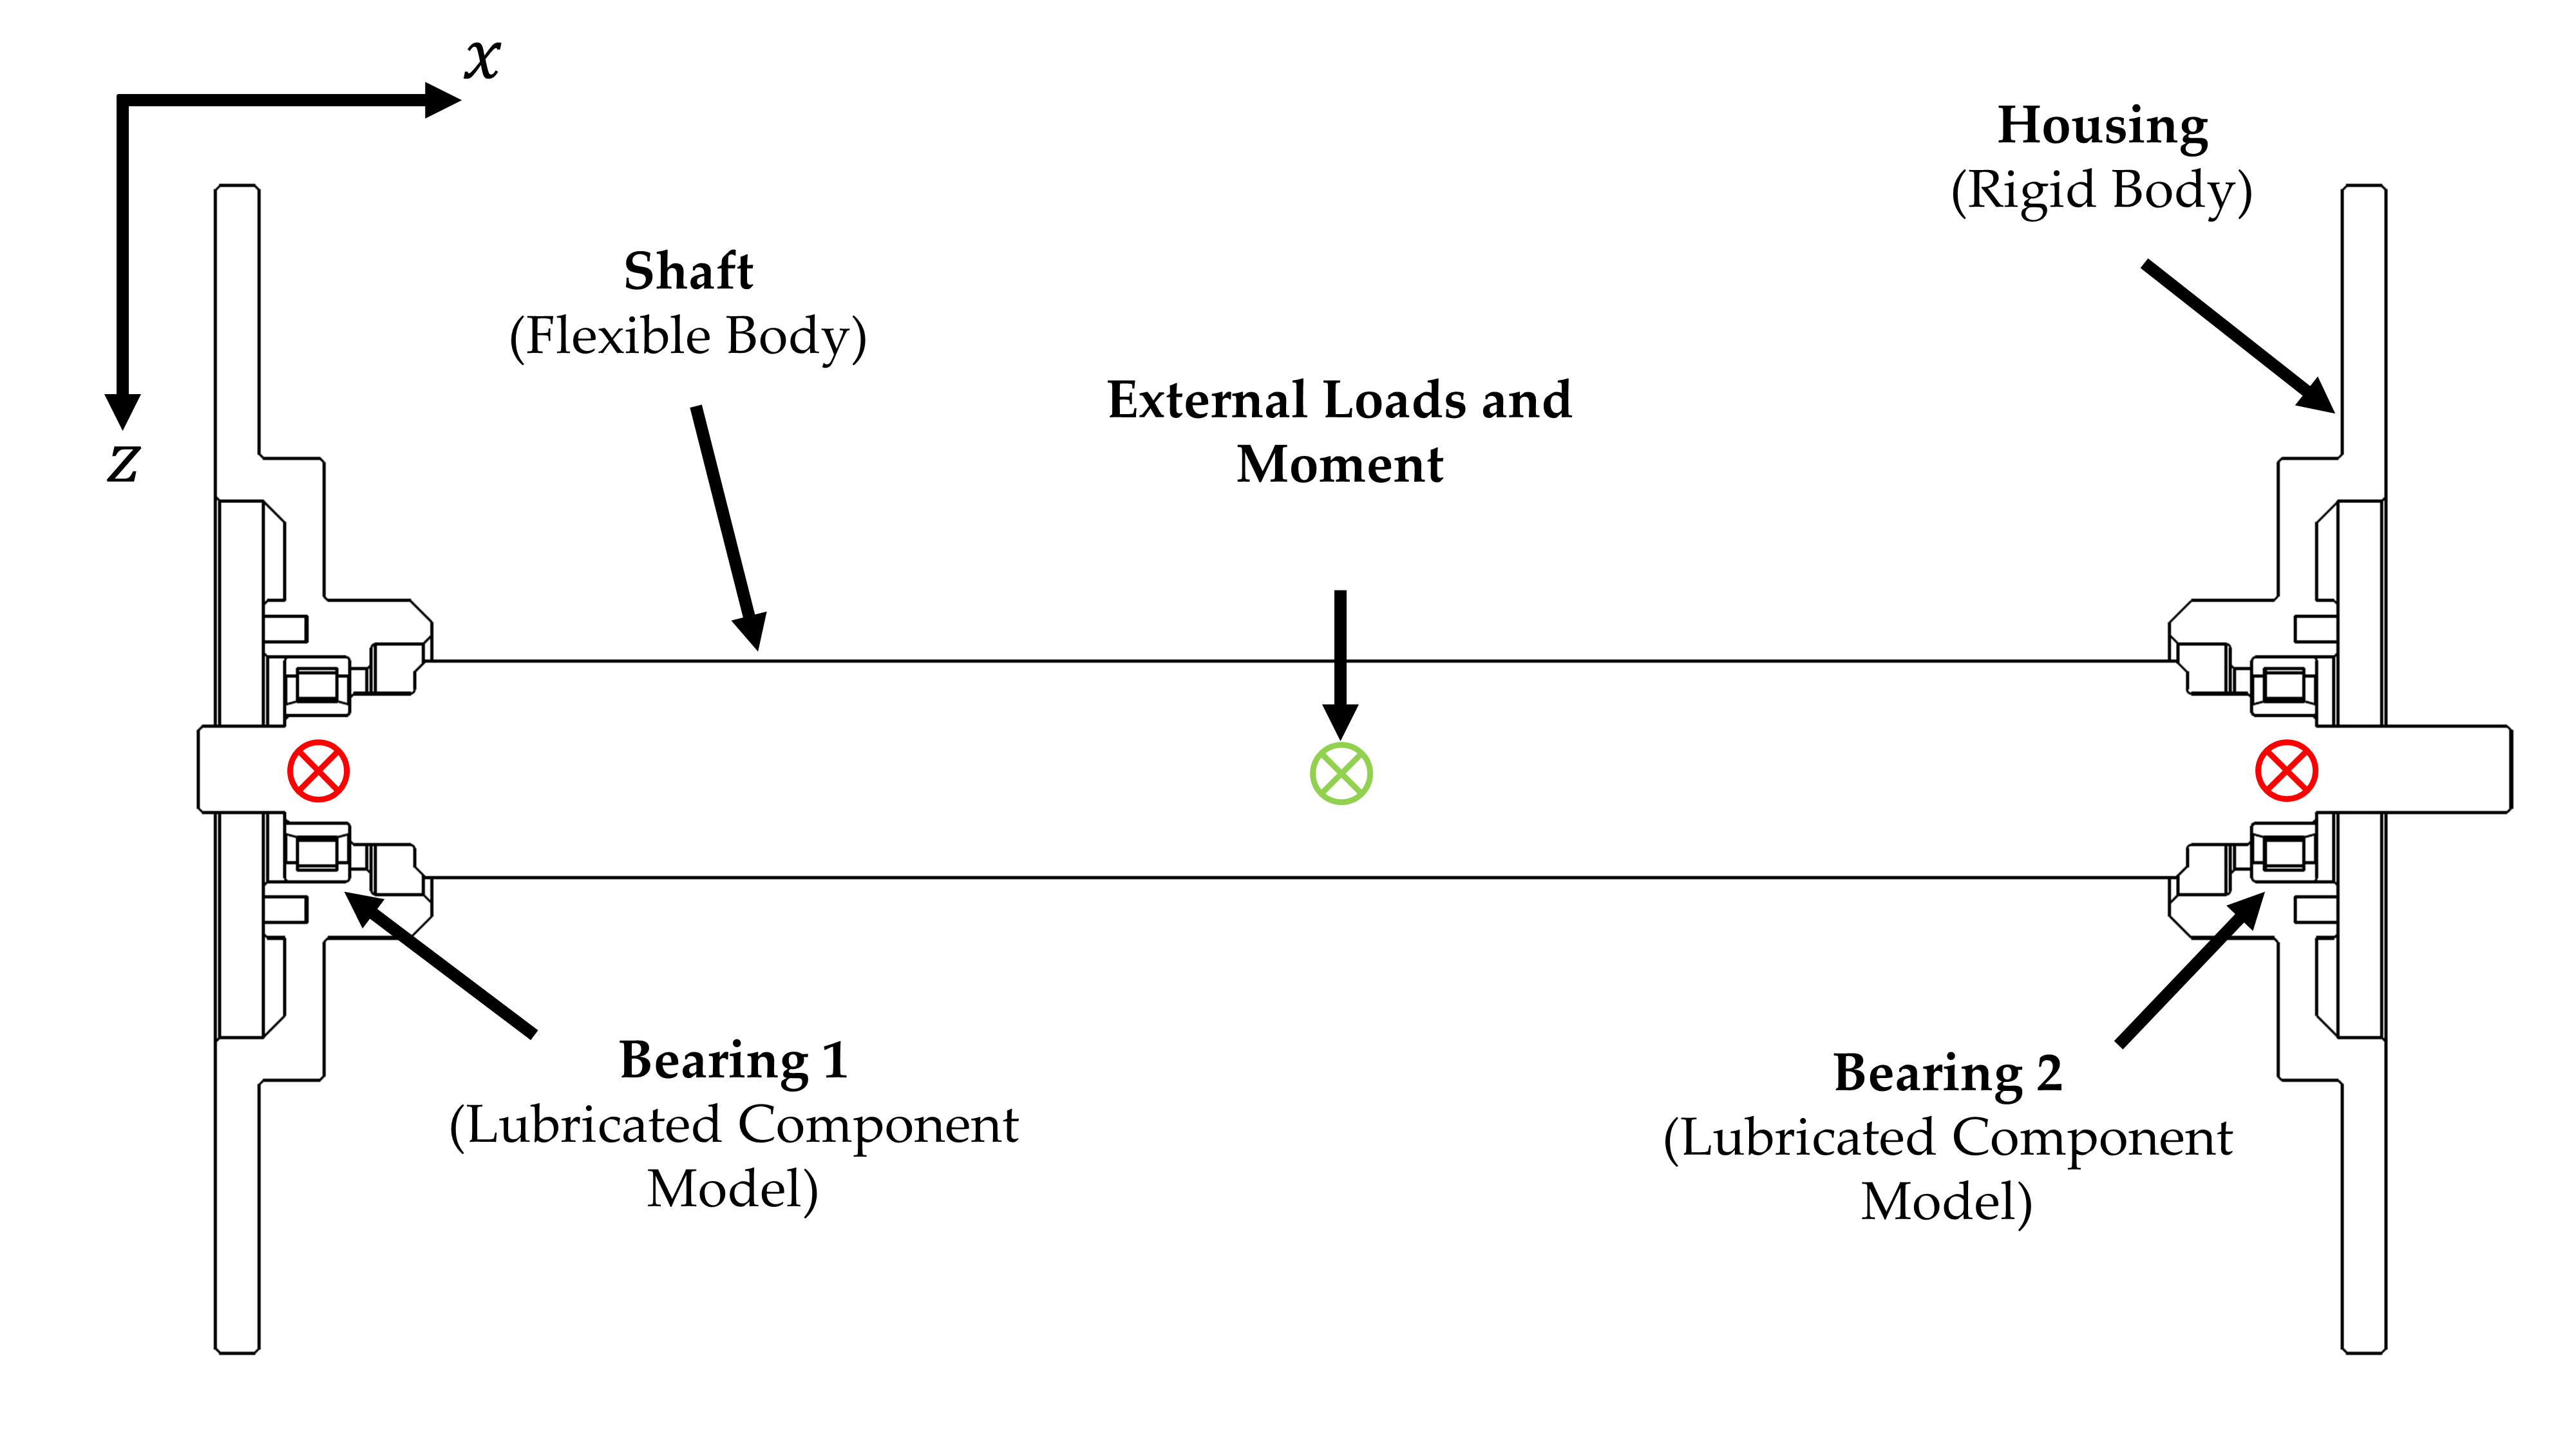
\includegraphics[width=150mm]{FlexiTribo Figure 2. System Level Model Schematic.png}
	\caption{System level model schematic.}
	\label{System level model schematic}
\end{figure} 

In typical configurations containing flexible structures, it is possible for both the inner and outer races of a rolling element bearing to move when subject to load. For this analysis, however, it is sufficient to fix the outer race in space and consider only the displacement of the inner bearing race \cite{DeMul1989_2}. The housing in this study is treated as a rigid body of infinite stiffness; therefore, the race dynamics of the bearing are influenced only by the motion of the flexible shaft in the model. The loading on the inner race is reacted by the rolling elements on the inner raceway; this must therefore be solved to achieve a dynamic equilibrium.

Within the model, the shaft is treated as a body having linear elastic behaviour and the housing is treated as rigid. The bearings are modelled via non-linear contact forces acting between the shaft and housing.

The shaft is represented by a condensed finite element model and is discretised into partial masses \cite{Parikyan2001}. The total elastic deformation of the shaft is represented by translational and rotational displacement components of these individual partial masses. The mathematical modelling used in the FMBD solver is based on Newton’s equations of motion and Euler’s equation of angular momentum, respectively:

\begin{equation}\label{NewtonFMBD}
	m_i \frac{\partial^2 x_i^{A b s}}{\partial t^2}=f_{F, i}^{A b s}
\end{equation}

\begin{equation}\label{EulerFMBD}
	\frac{\partial}{\partial t}\left(I_{C, i}^{A b s} \omega_i^{A b s}\right)=f_{M, i}^{A b s}
\end{equation}

where $m_i$ and $I_{C, i}^{A b s}$ represent the mass and inertia tensors of the partial masses, $i$. The vectors of displacement and angular velocity are represented by $x_i^{A b s}$ and $\omega_i^{A b s}$ respectively and are related to the centre of gravity of each partial mass. The force and moment vectors, $f_{F, i}^{A b s}$ and $f_{M, i}^{A b s}$, must be fulfilled for all partial masses in the shaft.

The combination of displacement and rotations of the shaft takes the form:

\begin{equation}\label{ShaftEquilibrium}
	M \ddot{q}=f
\end{equation}

where $M$ represents the block-diagonal mass matrix of the shaft, consisting of the sub-matrices $M_i, i \in\{1, \ldots, n\}$ that make up each partial mass of the full shaft. Acceleration, $\ddot{q}$, represents the second derivative of the displacement vector of all partial masses, $q=\left(q_1, q_2, \ldots, q_n\right)^t$. Each element of this vector has 6 elements associated with it that represent the 6 degrees of freedom - 3 rotational and 3 translational $\left(q_i=\right.$ $\left.\left(u_{t 1}, u_{t 2}, u_{t 3}, \emptyset_1, \emptyset_2, \emptyset_3\right)^t\right)$

The forces and moments acting on each partial mass are contained in sub-vectors of force, $f=\left(f_1, f_2, \ldots, f_n\right)^t$. These are split into a sum of internal force terms, $f_i^{i n t}$, external force terms, $f_i^{\text {ext }}$, and non-linear inertia terms, $p^*$. As with the partial mass terms, these are made up of six elements, each representing a degree of freedom:

\begin{equation}\label{Partial mass force}
	f_i^{i n t}=\left(\begin{array}{c}
		f_{i, 1}^{i n t} \\
		f_{i, 2}^{i n t} \\
		f_{i, 3}^{i n t} \\
		f_{i, 4}^{i n t} \\
		f_{i, 5}^{i n t} \\
		f_{i, 6}^{i n t}
	\end{array}\right)
\end{equation}

where each component of force, $f_{i, k}^{i n t}, k=1, \ldots, 6$ is evaluated using the linear-elastic approach

\begin{equation}\label{Partial mass force 6 dof}
	f_{i, k}^{i n t}=\sum_{j=1}^{6 . n} f_{i, j, k}^{i n t}
\end{equation}

\begin{equation}\label{Partial mass force 6 dof terms}
	f_{i, j, k}^{i n t}=-\left(d_{i, j, k} \dot{q}_k+k_{i, j, k} q_k\right)
\end{equation}

where $d$ and $\mathrm{k}$ represent the material damping and stiffness coefficients, respectively.

Grouping the damping and stiffness coefficients into one matrix gives the equation of motion after rearrangement. This equation represents the behaviour of the total system of rigid partial masses that make up the shaft, and considers both general global motion and small body motion (vibrations) \cite{Offner2011}:

\begin{equation}\label{Equation of motion}
	M \cdot \ddot{q}+D \cdot \dot{q}+K \cdot q=f^{e x t}+p^*
\end{equation}

The vector of external forces and moments, $f^{e x t}$, is the sum of excitation forces, $f^*$, and external loads, $f^a$. External loads and moments applied to the shaft, $f^a$, are determined functions given in time and are input as both time-varying and static loads on the system. The non-linear excitation force term, $f^*$, represents the reaction forces from the lubricated component level bearing model.

\begin{equation}\label{External forces}
	f^{e x t}=f^*+f^a
\end{equation}

Partial mass displacements $\left(q_i\right)$ and velocities $\left(\dot{q}_i\right)$ at the bearing locations are output from the dynamic model and used as boundary conditions within the lubricated component level bearing model at each time step of the simulation. This model returns resultant forces and torques on the inner race of each bearing $\left(f_i^*\right)$ which are then used to solve the equation of motion (Equation \ref{Equation of motion}) within the dynamic model (see Figure \ref{Flowchart of models}).

\subsection{Lubricated Component Level Model} \label{Contact mechanics FMBD}
The displacement and velocity vectors from each node connecting the shaft to the bearings $\left(q_i\right.$ and $\dot{q}_i$ respectively) comprise six-DOF. For this lateral DOF model, translations in $z$ and $y$ are considered, as well as angular displacement around the rotational axis, $x$. A schematic of the bearing is shown in Figure \ref{Bearing schematic}.

\begin{figure}
	\centering  
	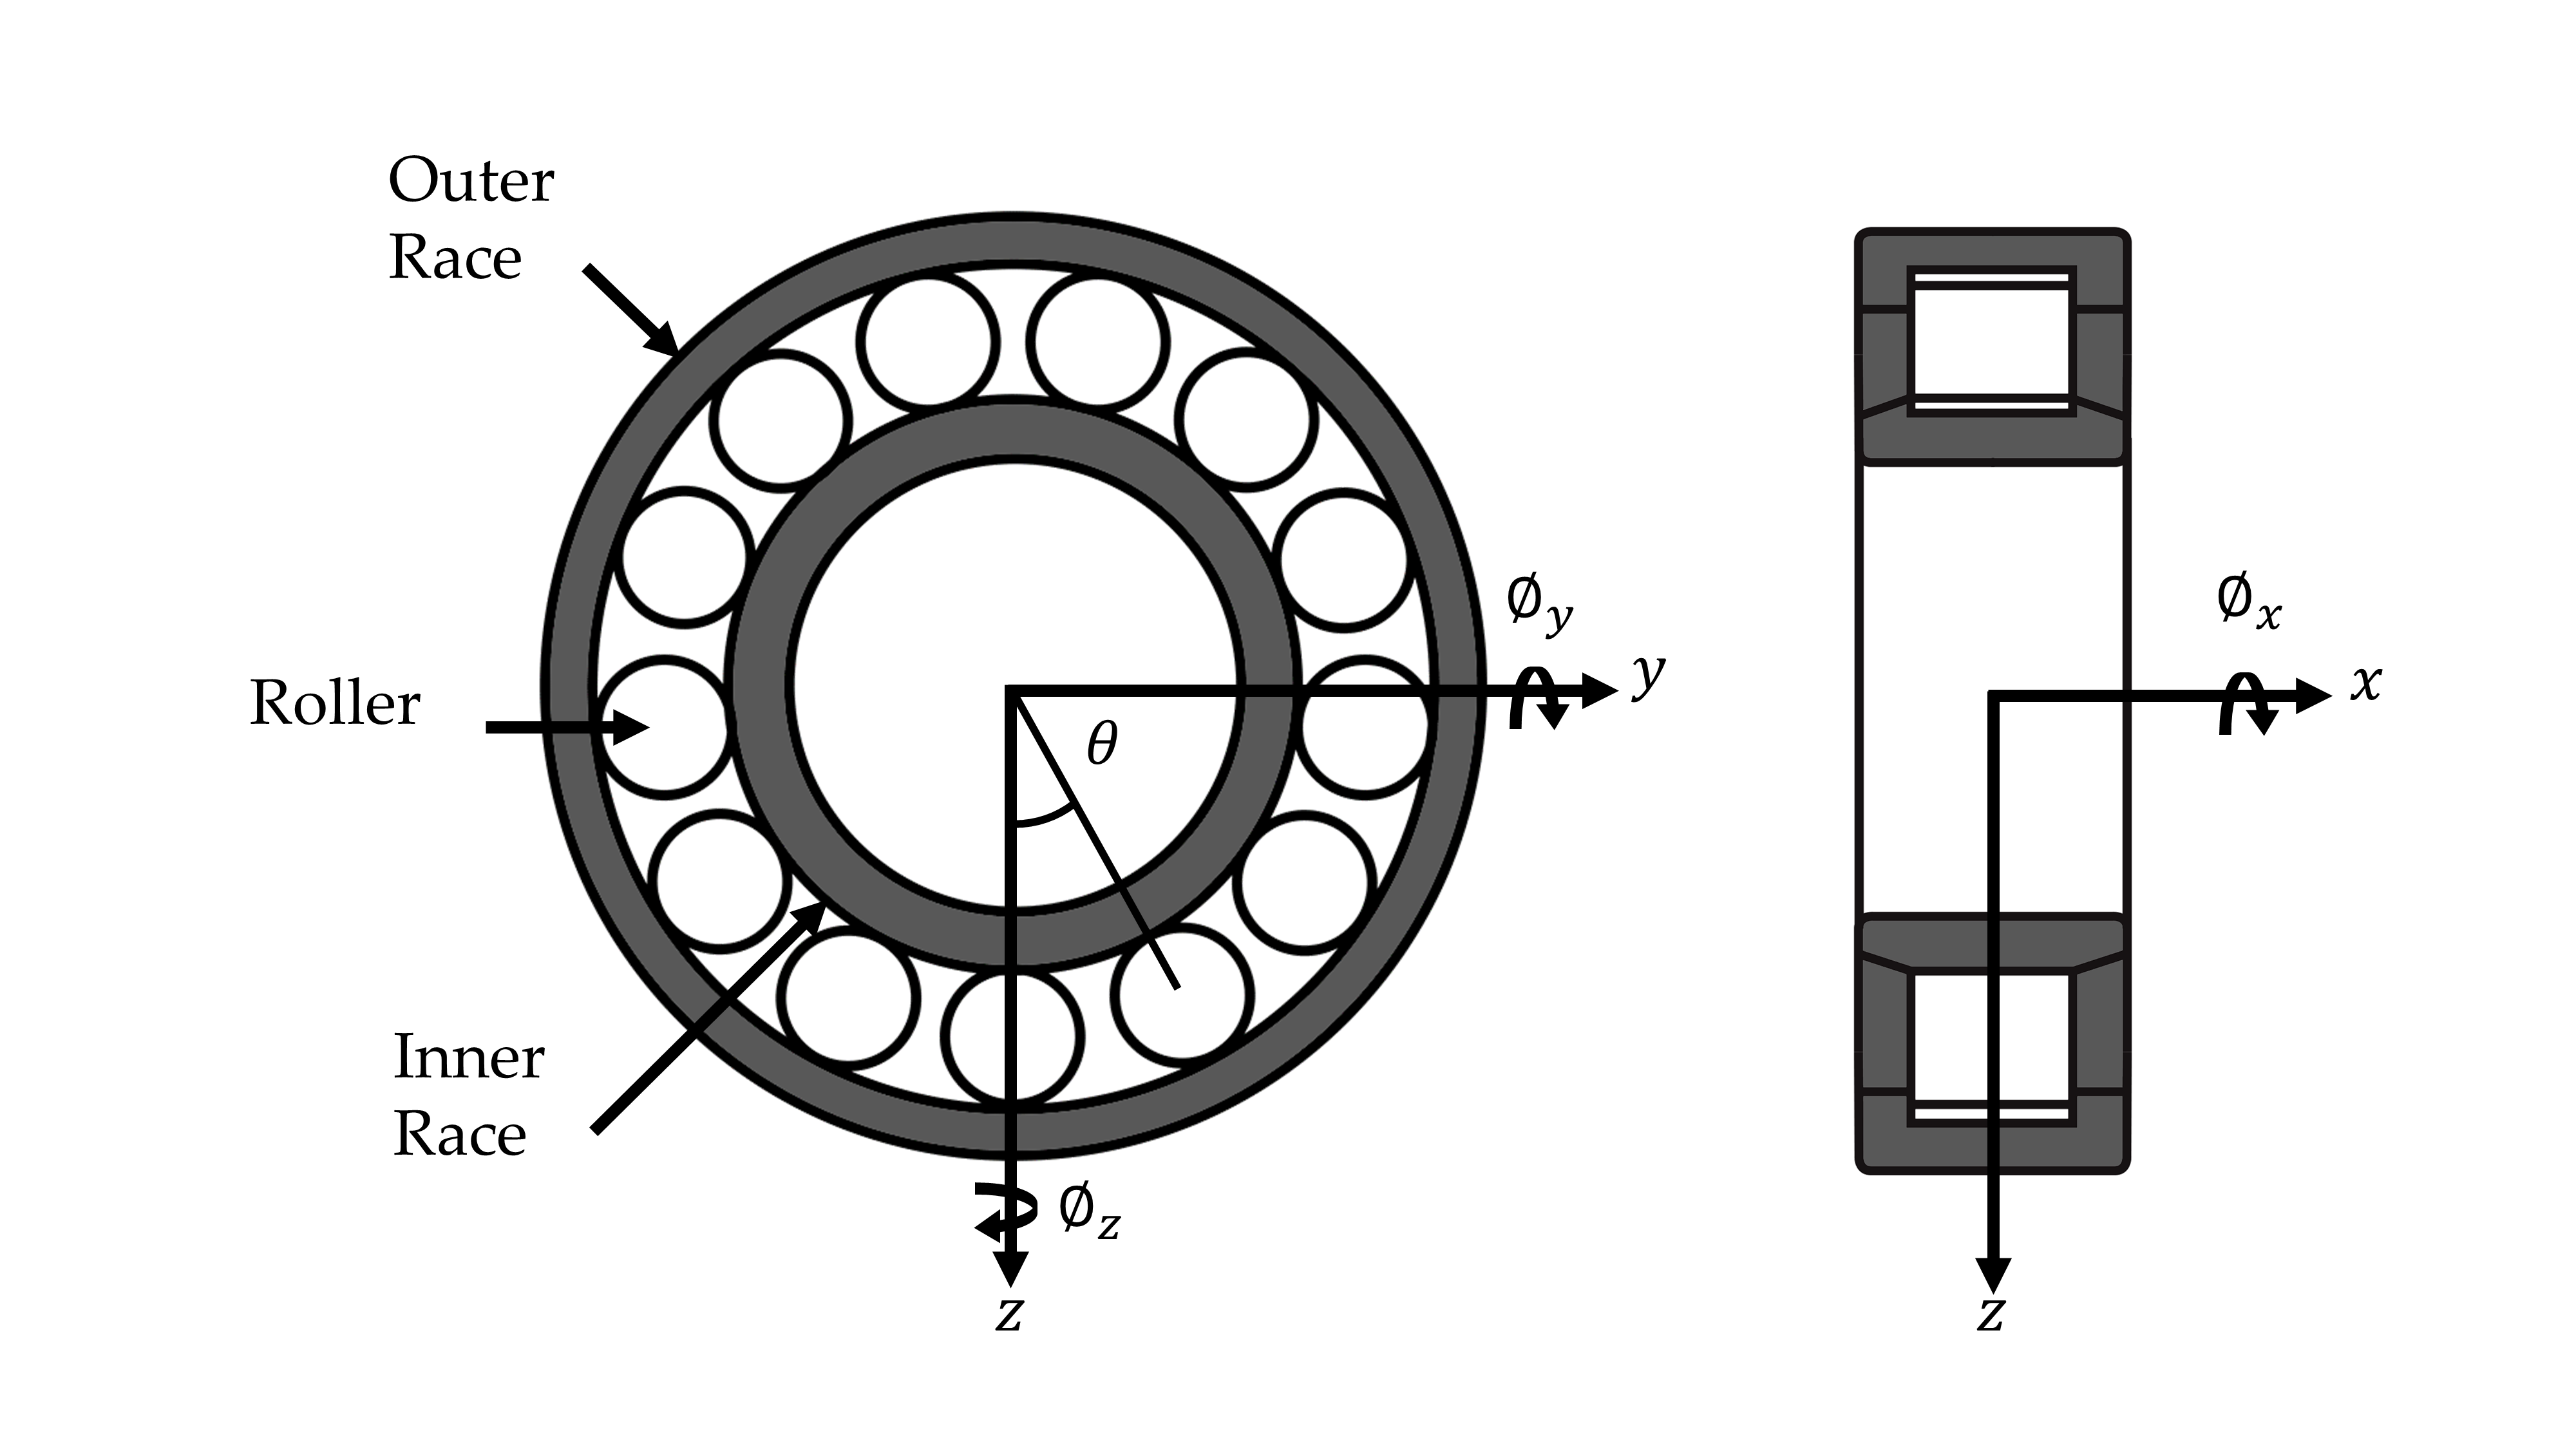
\includegraphics[width=150mm]{FlexiTribo Figure 3. Bearing Schematic.png}
	\caption{Bearing schematic.}
	\label{Bearing schematic}
\end{figure} 

Between the roller and raceways, under sufficient load, the pressures in the non-conformal contact are high enough to cause elastic deformation of the surfaces and a significant increase in lubricant viscosity. This, combined with relative motion between contacting bodies, leads to the generation of an EHL contact. The stiffness of the EHL film is typically 1-2 orders greater than the stiffness of the contacting bodies \cite{Dietl1997}. In this analysis, the film stiffness was calculated using:

\begin{equation}\label{Film stiffness}
	K_{E H L}=\frac{d w}{d h_c}
\end{equation}

The lowest average film stiffness was $5.1 \times 10^9 \mathrm{~N} / \mathrm{m}$, which is over one order greater than the contacting material stiffness. The material therefore dominates the stiffness of the contact, and the stiffness of the EHL film can be neglected. The film is modelled as a rigid element that is present between the roller and race \cite{Walford1983} \cite{Dareing1975} \cite{Mehdigoli1990}.

The contact deformation $(\delta)$ is therefore a function of the displacement of the inner bearing race, angular displacement of the roller about the rotational axis $(\theta)$, central EHL film thickness $\left(h_c\right)$ and any clearance or radial preload $( \pm C)$ within the bearing \cite{Rahnejat1985} \cite{Mohammadpour2015c}:

\begin{equation}\label{Contact deformation flextribo}
	2 \delta=2\left(h_c-C\right)+z \cos (\theta)+y \sin (\theta)
\end{equation}

Figure \ref{Dry vs lubricated roller-race contact} demonstrates this more clearly. The total contact deformation is the summation of $\left(h_c\right)$ and the material deformation, $\left(\delta_m\right)$ predicted from the dry-Hertzian contact assumption. Conventional dry analysis only accounts for the dry material deformation at the contact.

\begin{figure}
	\centering  
	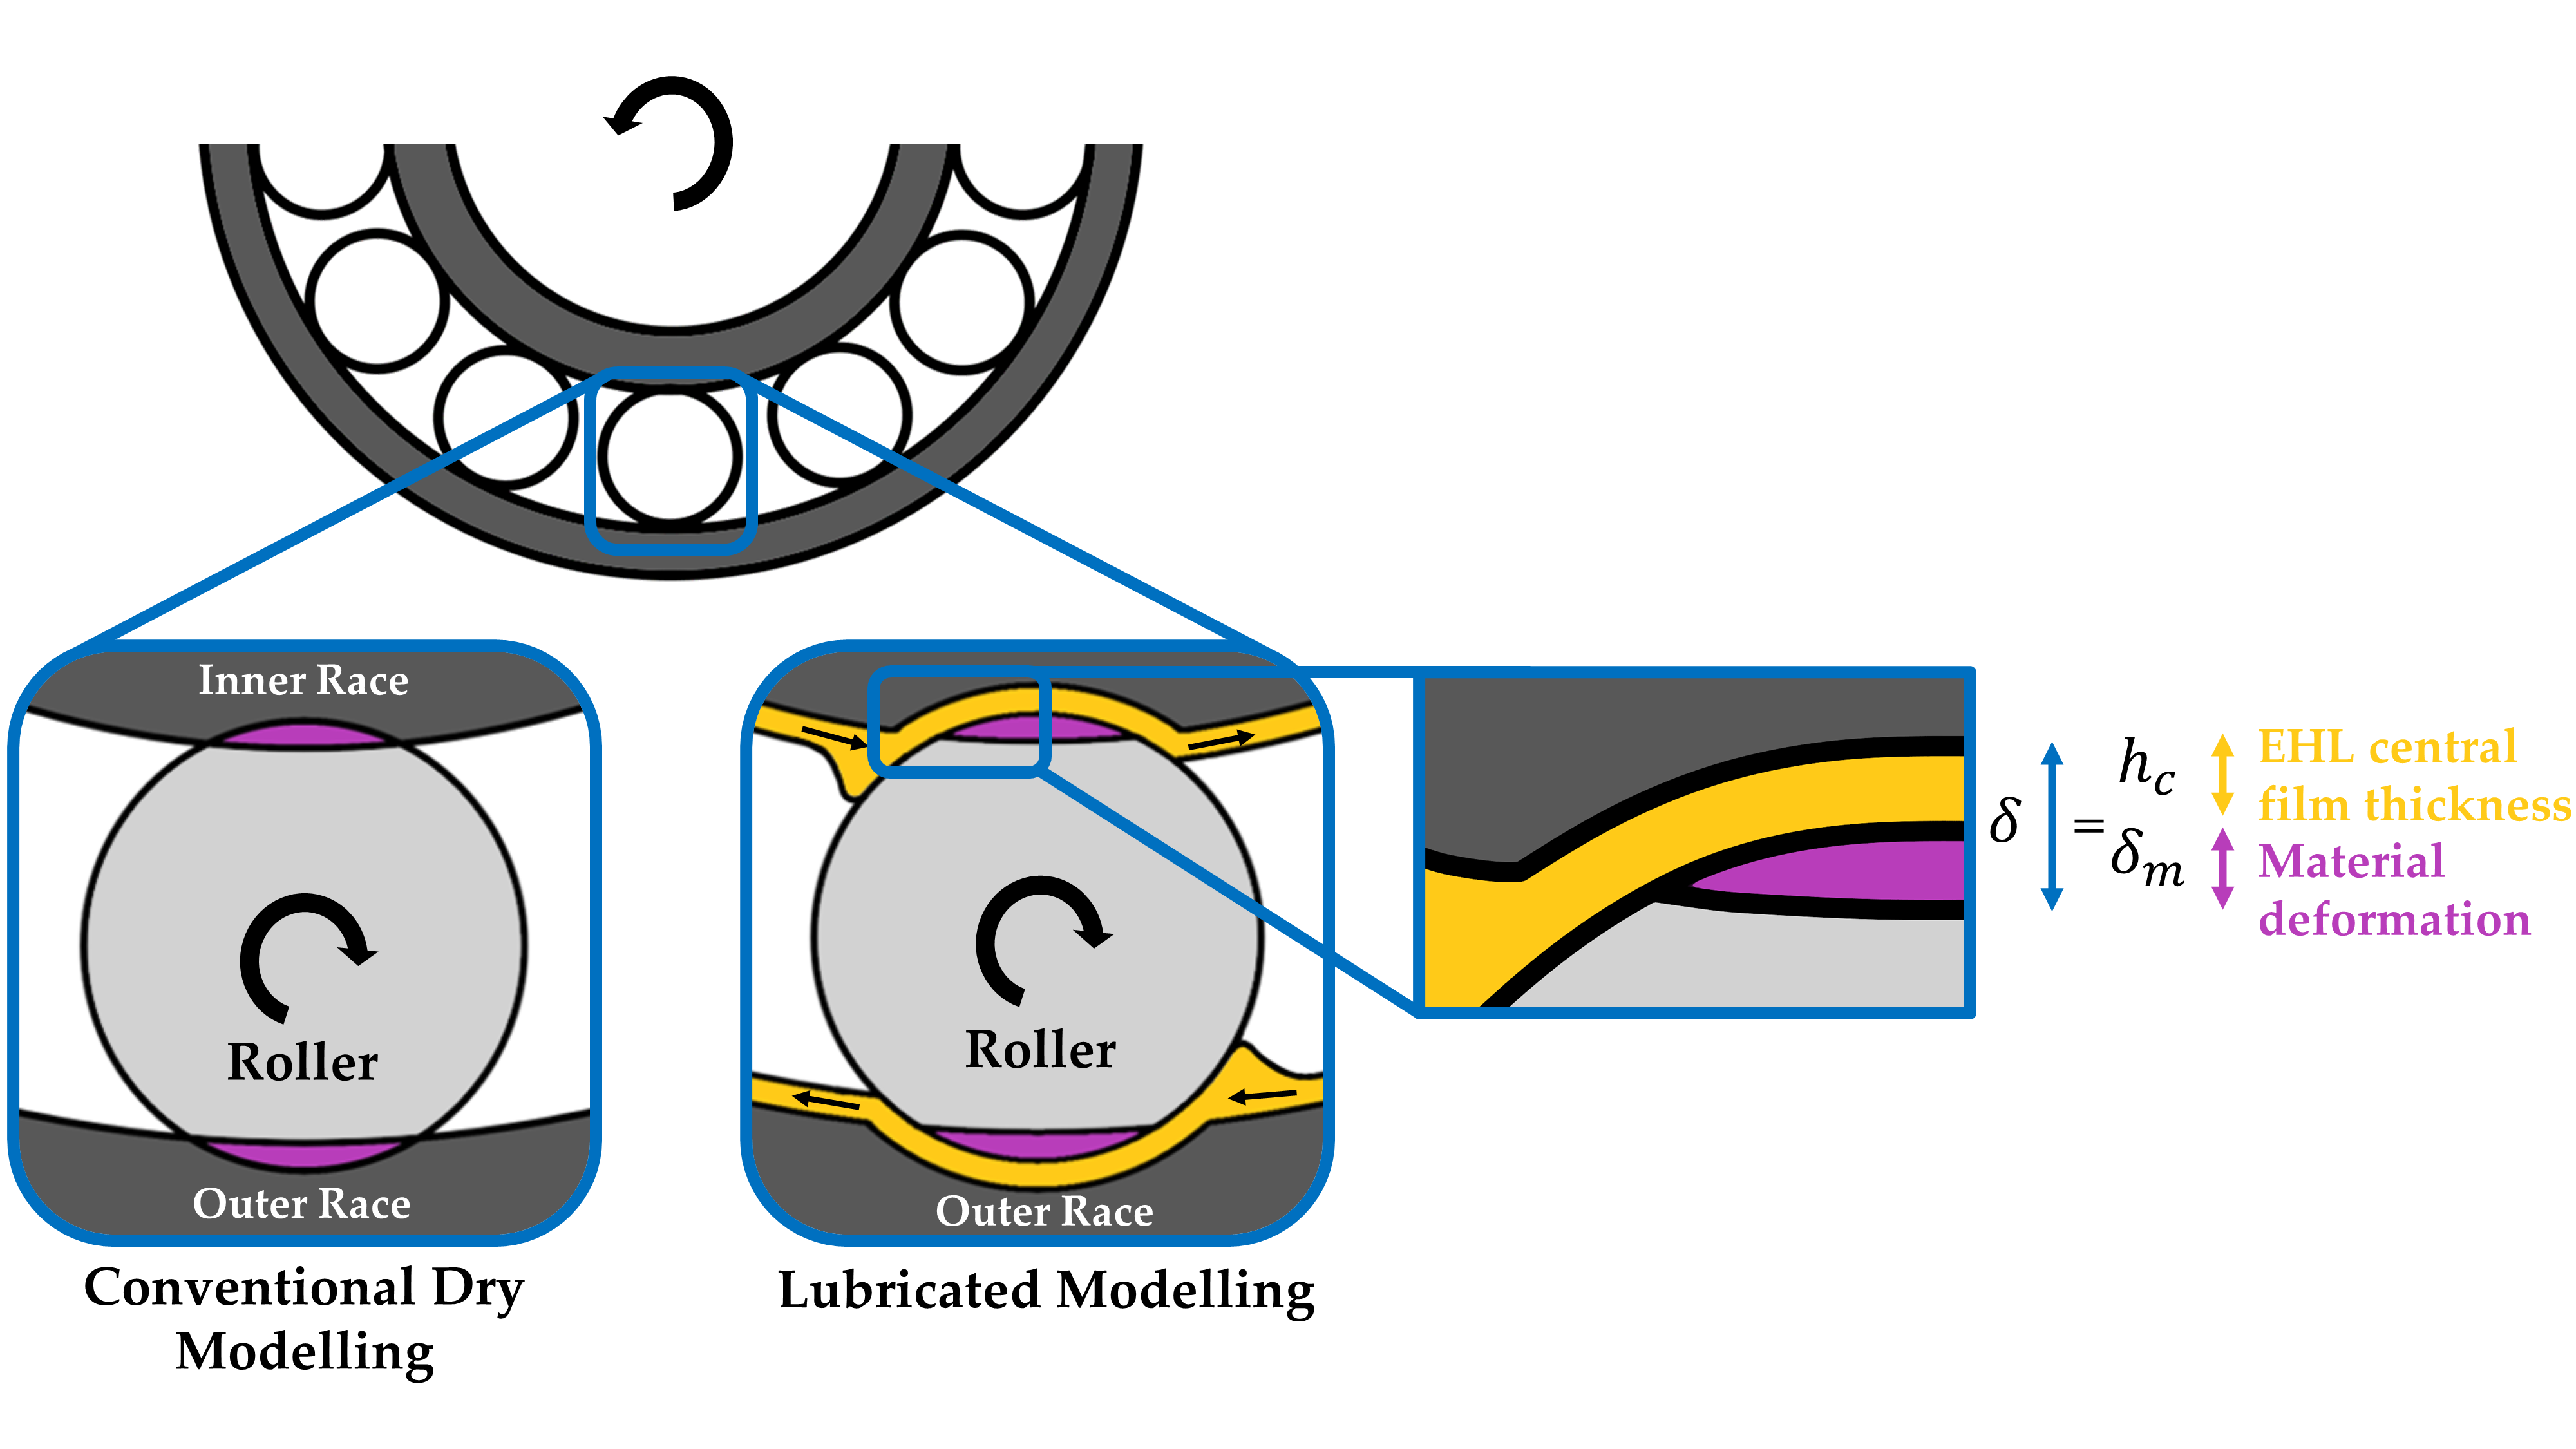
\includegraphics[width=150mm]{FlexiTribo Figure 4. Dry vs Lubricated Roller-Race Contact.png}
	\caption{Dry vs lubricated roller-race contact.}
	\label{Dry vs lubricated roller-race contact}
\end{figure} 

The extrapolated central film thickness for a line contact, assuming a fully flooded contact inlet, is therefore obtained from \cite{Dowson1979}: 

\begin{equation}\label{DowsonToyodaCentralFilm}
	h_c=R_r\left[3.06 G^{* 0.56} U^{* 0.69} W^{*-0.1}\right]
\end{equation}

where the following dimensionless parameters are used:

\begin{equation}\label{DowsonToyodaDimensionless}
	W^*=\frac{W}{E_r R_r l_a}, U^*=\frac{\eta_0 U}{E_r R_r}, G^*=E_r \alpha
\end{equation}

Comprehensive analytical models \cite{Nelias2008} \cite{Majdoub2020} account for the tilting and skew of the rolling elements. Skew has the effect of varying the entrainment speed along the length of the roller, and tilt will affect the contact gap. Due to the stiff housing and shaft used in this analysis, the tilt and skew angles are very small. The entraining motion and contact gap along the contact length can be considered consistent, and a 1D analysis for EHL film thickness is therefore appropriate \cite{Gupta1979}.

The bearings are modelled with light preload due to mounting interference. In practical applications, preload is applied to prevent skidding and chaotic behaviour due to the emergence of zero stiffness regions \cite{Mevel1993}. In contrast, excessive preload can lead to frictional power loss and wear. Assuming pure rolling, the speed of entraining motion is given by \cite{Spikes2015} \cite{Shi2015}: 
	
\begin{equation}\label{SpikesEntrainmentSpeed}
	u=\frac{R \omega}{r}\left(\frac{(R+2 r)}{(R+r)}\right)
\end{equation}

Due to the dependency of load on film thickness, an iterative approach is performed to calculate the contact force. Convergence criteria for the EHL film must be met at each time step of the simulation before the bearing forces are returned to the system level model and the equations of motion are solved:

\begin{equation}\label{FilmConvergence}
	\frac{h_c^m-h_c^{m-1}}{h_c^{m-1}} \leq 0.001
\end{equation}

where $m$ represents the iteration number.

Individual roller-race contact forces are calculated based on the contact deformation. In the case of a rolling element, a cylindrical body of finite length, the contact problem is non-Hertzian. The surfaces cannot be modelled as locally quadratic due to the presence of crowned (rounded) edges \cite{Singh1974}. The most widely used technique to calculate the force-deflection relationship is the contact slicing technique. Whilst this does not reflect edge stress concentrations, these stresses are only distributed over a small area and hence can be neglected for the purpose of force equilibrium \cite{Harris2007a}. In general, this technique is favoured for its simplicity, speed, and sufficient accuracy. The contact slicing technique employed in this study was developed by Andreason \cite{Andreason1973} for modelling these non-Hertzian line contacts.
 
Modelling the roller-race contacts as a line contact between a cylindrical roller and a flat surface, Lundberg’s \cite{Lundberg1949} expression between contact force per unit length ($w$) and deformation ($\delta$) was used. 

\begin{equation}\label{Lundberg deflection}
	\frac{\delta}{l_a}=\frac{2 w}{\pi E_r l_a} \ln \frac{\pi E_r l_a}{w}
\end{equation}

where $E_r$ is the equivalent elastic modulus of the two materials and $l_a$ is the active length of the roller. This assumes that the pressure distribution is uniform along the length of the contact, and elliptical across it. This neglects side leakage along the contact $\left(x_c\right)$ due to the contact dimensions in this direction being much larger than dimensions across it $\left(y_c\right)$. This is valid apart from the small regions at the edges of the contact.

From Equation \ref{Lundberg deflection}, contact forces per unit length of an individual slice along the roller-race contact can be calculated. This is valid if there is no separation of the bodies, i.e., the contact deformation does not become negative $\left(\delta_k>0\right)$.

\begin{equation}\label{Contact force per unit length Lundberg}
	w_s=\pi E_r l_s\left(\frac{0.5 \delta_s}{7.358 l_s}\right)^{1.11}
\end{equation}

where $s$ represents the slice number, and $l$ represents the slice length.

The application of the slicing technique was validated against open literature \cite{DeMul1989_2}. The study compared results obtained from an experimental rig with numerical results calculated using both the approximate slicing technique and the sophisticated non-Hertzian technique \cite{DeMul1986}. By replicating the geometry of the test bearing used in their analysis, the application of Andreason’s slicing technique used for this analysis was validated with good agreement (see Figure \ref{Contact level validation}). This method is a much faster way of calculating contact load and moment than more sophisticated methods by \cite{DeMul1989_2}, yet still maintains high accuracy.

\begin{figure}
	\centering  
	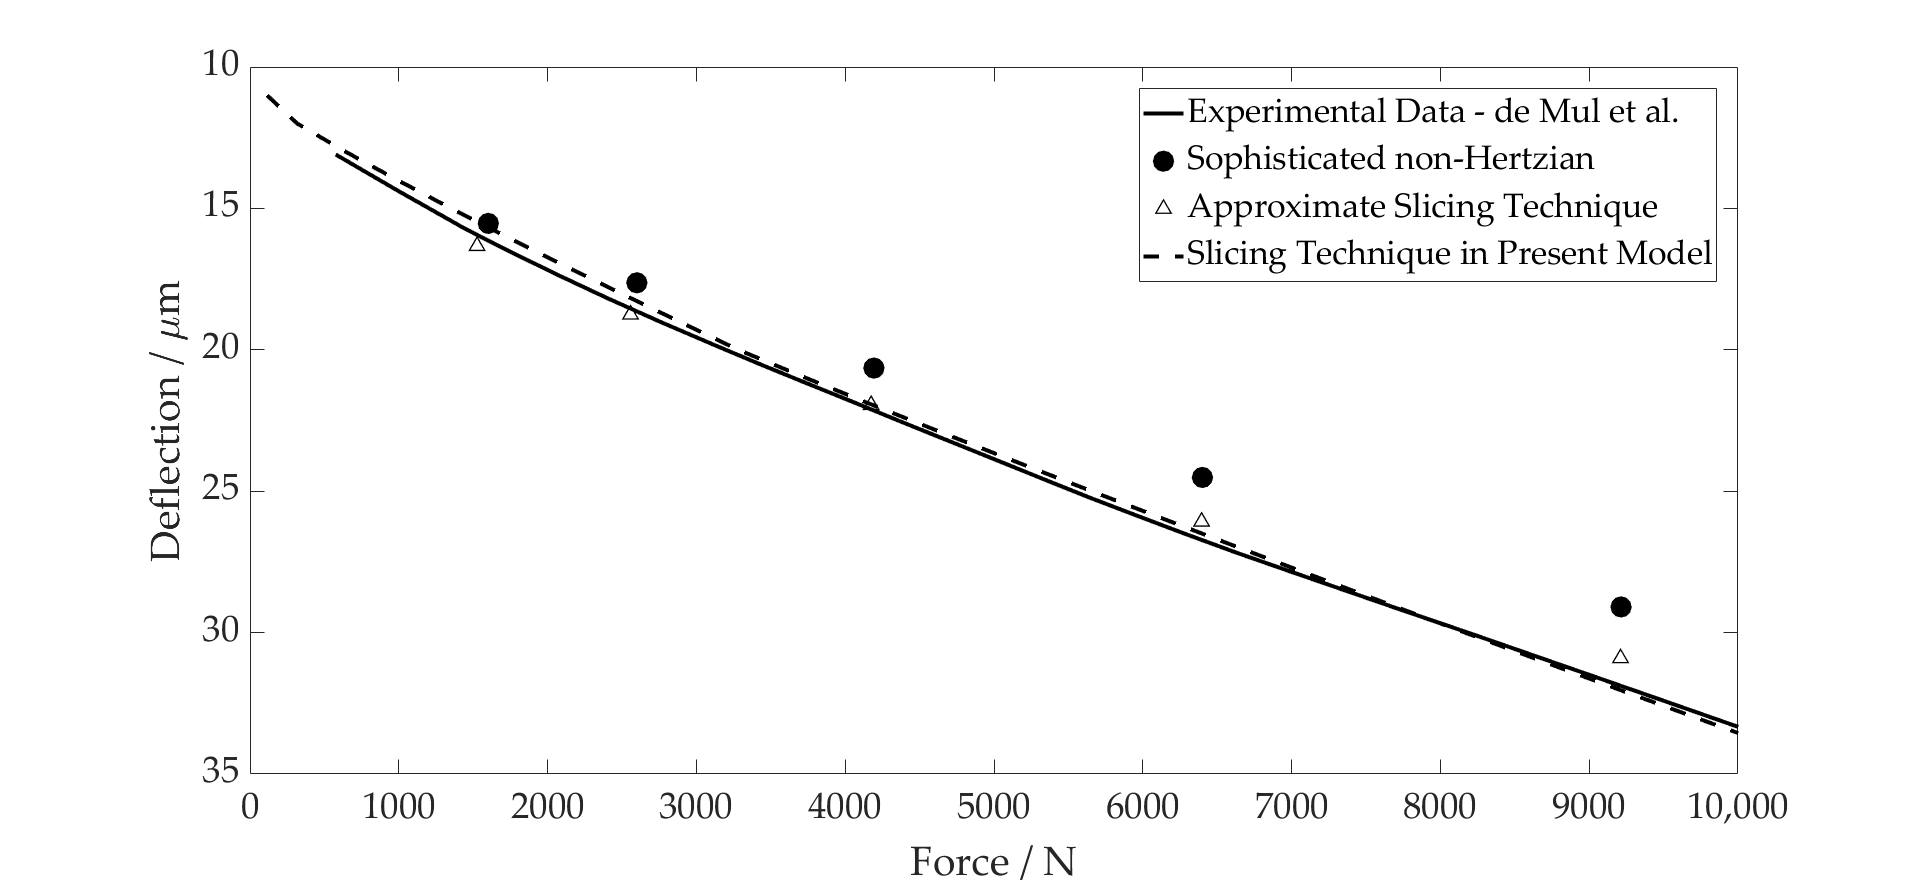
\includegraphics[width=150mm]{FlexiTribo Figure 5. Contact Level Validation.png}
	\caption{Contact level validation.}
	\label{Contact level validation}
\end{figure} 

The total contact load $W$ and moment $T$ are obtained by summing the contributions from all loaded slices:

\begin{equation}\label{Total contact load flexitribo}
	W=\sum_s w_s l_s
\end{equation}

\begin{equation}\label{Total contact torque flexitribo}
	T=\sum_s w_s l_s x_{c, s}
\end{equation}

with $x_{c, s}$ being the distance to the centre of each slice in the conjunction coordinate system. It is assumed that total contact deflection is shared equally between the inner and outer races despite slight differences in contact geometry. The entrainment velocity is equal at each contact, which is the governing parameter for the lubricated contact force differences.

Experimental measurements show that the damping of a rolling element bearing arises from multiple sources \cite{Dietl1997}, including:
 
\begin{enumerate}
	\item Lubricant film damping at the contacts.
	\item Material damping due to Hertzian deformations.
	\item Interface damping between assembled components
\end{enumerate}

These measurements show that damping decreases with rotational speed, tending towards a constant value. Sopanen and Mikkola \cite{Sopanen2003_1} summarize the findings of Mitsuya et al. \cite{Mitsuya1992} and Aini et al. \cite{Aini2002}, concluding that the film damping is moderate. The linearized viscous damping method adopted in their study is therefore also adopted here. The damping force for each roller is obtained as a factor of the contact stiffness and contact penetration velocity \cite{Kramer1993}. This is defined as:

\begin{equation}\label{Kramer damping}
	\left|F_d\right|=-f_{\text {damp }} K_c \dot{q}
\end{equation}

where $K_c$ is the contact stiffness, and the damping factor, $f_{\text {damp}}$, is in the range of $(0.25-2.5) \times 10^{-5}$ as reported by \cite{Kramer1993}.

At each time step of the analysis, these calculations are performed for each individual roller in the complement. The total bearing force acting on the inner race is solved by splitting the total contact force on each roller into its components and summing their contributions.

\begin{equation}\label{Total bearing force z flexitribo}
	f_{z, i}^*=\sum_N W \cos (\theta)-\sum_N F_d \cos (\theta)
\end{equation}

\begin{equation}\label{Total bearing force y flexitribo}
	f_{y, i}^*=\sum_N W \sin (\theta)-\sum_N F_d \sin (\theta)
\end{equation}

Due to the bearing preload, contact is maintained throughout the rollers’ orbit; hence no emerging clearances are modelled in the lubricated analysis. The contact separation is also unaffected by rolling element centrifugal forces, which are negligible when compared to the contribution of the dynamic load and the EHL film in this study. These have therefore been neglected.

Surface measurements of the rollers used in this analysis were taken using an Alicona InfiniteFocus Variation Microscope (see Section \ref{Surface Topography}) . The composite surface roughness value of a roller and inner race was calculated to be 0.207~$\mu m$. This gives a lambda value of 2.59 for the thinnest EHL film at 1000~$rpm$. Asperity interaction is not considered as the EHL film fully supports the load. Due to the pure rolling and zero sliding assumption, friction at the contacts is therefore neglected and the analysis is performed under isothermal conditions. 

The bearing geometry is detailed in Table \ref{Cylindrical Roller Bearing Specification}. Rheological and material properties are detailed in Table \ref{Bearing Rheological Properties}, representing ambient operating conditions in an individual hub-motor transmission. 

\begin{table*}
	%\captionsetup{justification=centering}
	\caption{Cylindrical Roller Bearing Specification}
	\label{Cylindrical Roller Bearing Specification}
	\centering
	\renewcommand{\arraystretch}{1.5}%
	\begin{tabular}{|c|c|}
		\hline
		\ \textbf{Parameter} & \textbf{Value} \\ [0.5ex]
		\hline
		Inner race bore diameter & 25 $mm$ \\ [0.5ex]
		\hline
		Pitch diameter & 60 $mm$ \\ [0.5ex]
		\hline
		Roller diameter & 8.8 $mm$ \\ [0.5ex]
		\hline
	    Roller length & 15 $mm$ \\ [0.5ex]
		\hline
	    Number of rollers & 17 \\ [0.5ex]
		\hline
		Operating clearance & -2 $\mu \mathrm{m}$ \\ [0.5ex]
		\hline
	\end{tabular}
\end{table*}

\begin{table*}
	%\captionsetup{justification=centering}
	\caption{Bearing Material and Rheological Properties}
	\label{Bearing Rheological Properties}
	\centering
	\renewcommand{\arraystretch}{1.5}%
	\begin{tabular}{|c|c|}
		\hline
		\ \textbf{Parameter} & \textbf{Value} \\ [0.5ex]
		\hline
		Pressure viscosity coefficient ($\alpha$) & 2.1 $\times 10^{-8}\mathrm{~Pa}^{-1}$ \\ [0.5ex]
		\hline
		Atmospheric lubricant dynamic viscosity & 0.08 Pa.s \\ [0.5ex]
		\hline
		Lubricant inlet density ($\rho_0$) & 833.8 $\mathrm{~kg}\cdot\mathrm{m}^{-3}$ \\ [0.5ex]
		\hline
		Modulus of elasticity of contacting solids & 210 GPa \\ [0.5ex]
		\hline
	    Poisson’s ratio of contacting solids & 0.3 \\ [0.5ex]
		\hline
	\end{tabular}
\end{table*}

\subsection{Representative Excitation Methodology}

The system level model is decomposed, with excitation forces calculated externally before application within the model. A separate electrified transmission model is used to generate realistic excitation forces and torques from a spur gear pair and a permanent magnetic synchronous motor (PMSM). This system represents the first stage of an electric hub motor used in automotive applications.

\begin{figure}
	\centering  
	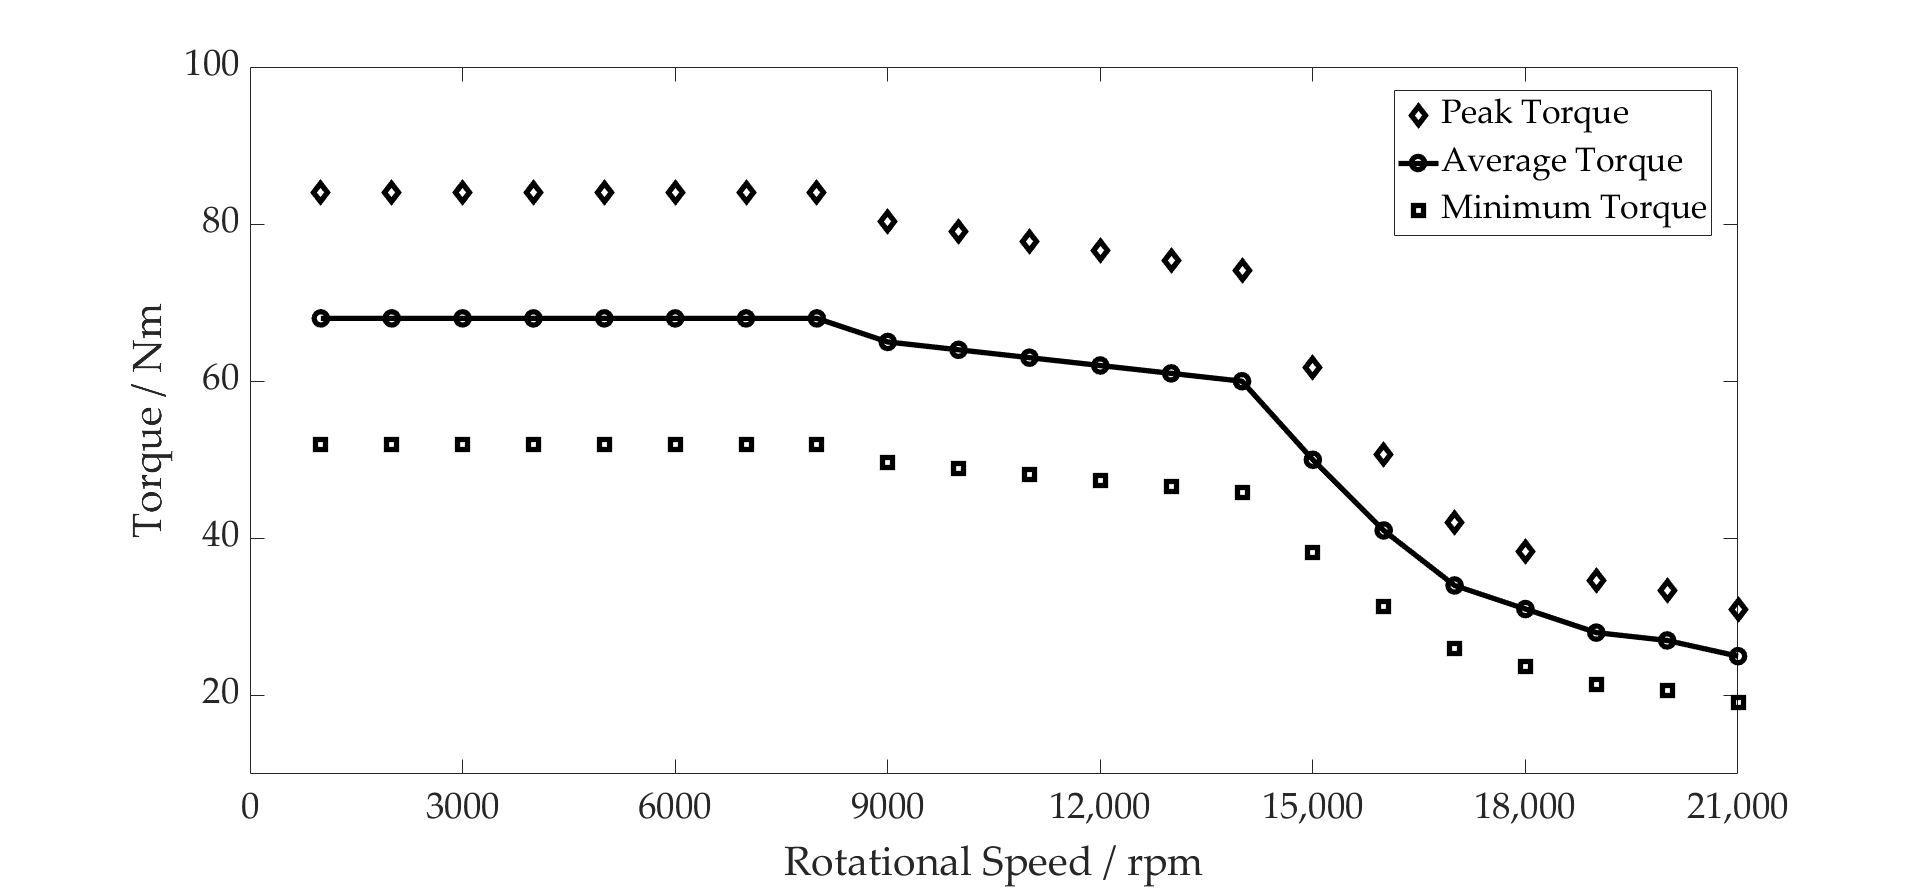
\includegraphics[width=150mm]{FlexiTribo Figure 6. PMSM Torque Profile and Maximum and Minimum Torque Fluctuation.png}
	\caption{PMSM torque profile and maximum and minimum torque fluctuation.}
	\label{PMSM torque profile}
\end{figure} 

Radial and tangential gear pair forces at the pinion centre, as well as torque fluctuations of the electric motor are extracted to be used as inputs to the system level model. These are applied as external forces to the shaft, $f^a$, from Equation \ref{External forces}. All bodies in this separate system were modelled as rigid, so that structural excitation forces did not contribute to the resultant forces at the pinion.

The motor has a peak torque of 68~$\mathrm{Nm}$, and a maximum operating speed of 21~000~$\mathrm{rpm}$. The torque transfer through the gear pair reduces as the speed increases due to the torque profile of the PMSM, as shown in Figure \ref{PMSM torque profile}. Stator tooth forces from the PMSM are neglected in the model due to their minimal contribution to lateral forces once resolved. For input to the model, the radial and normal forces are simplified by adopting sinusoidal inputs of the same magnitude and frequency of the gear pair at different speeds. The torque ripple from the motor is simplified using the same method.

\begin{figure}
	\centering  
	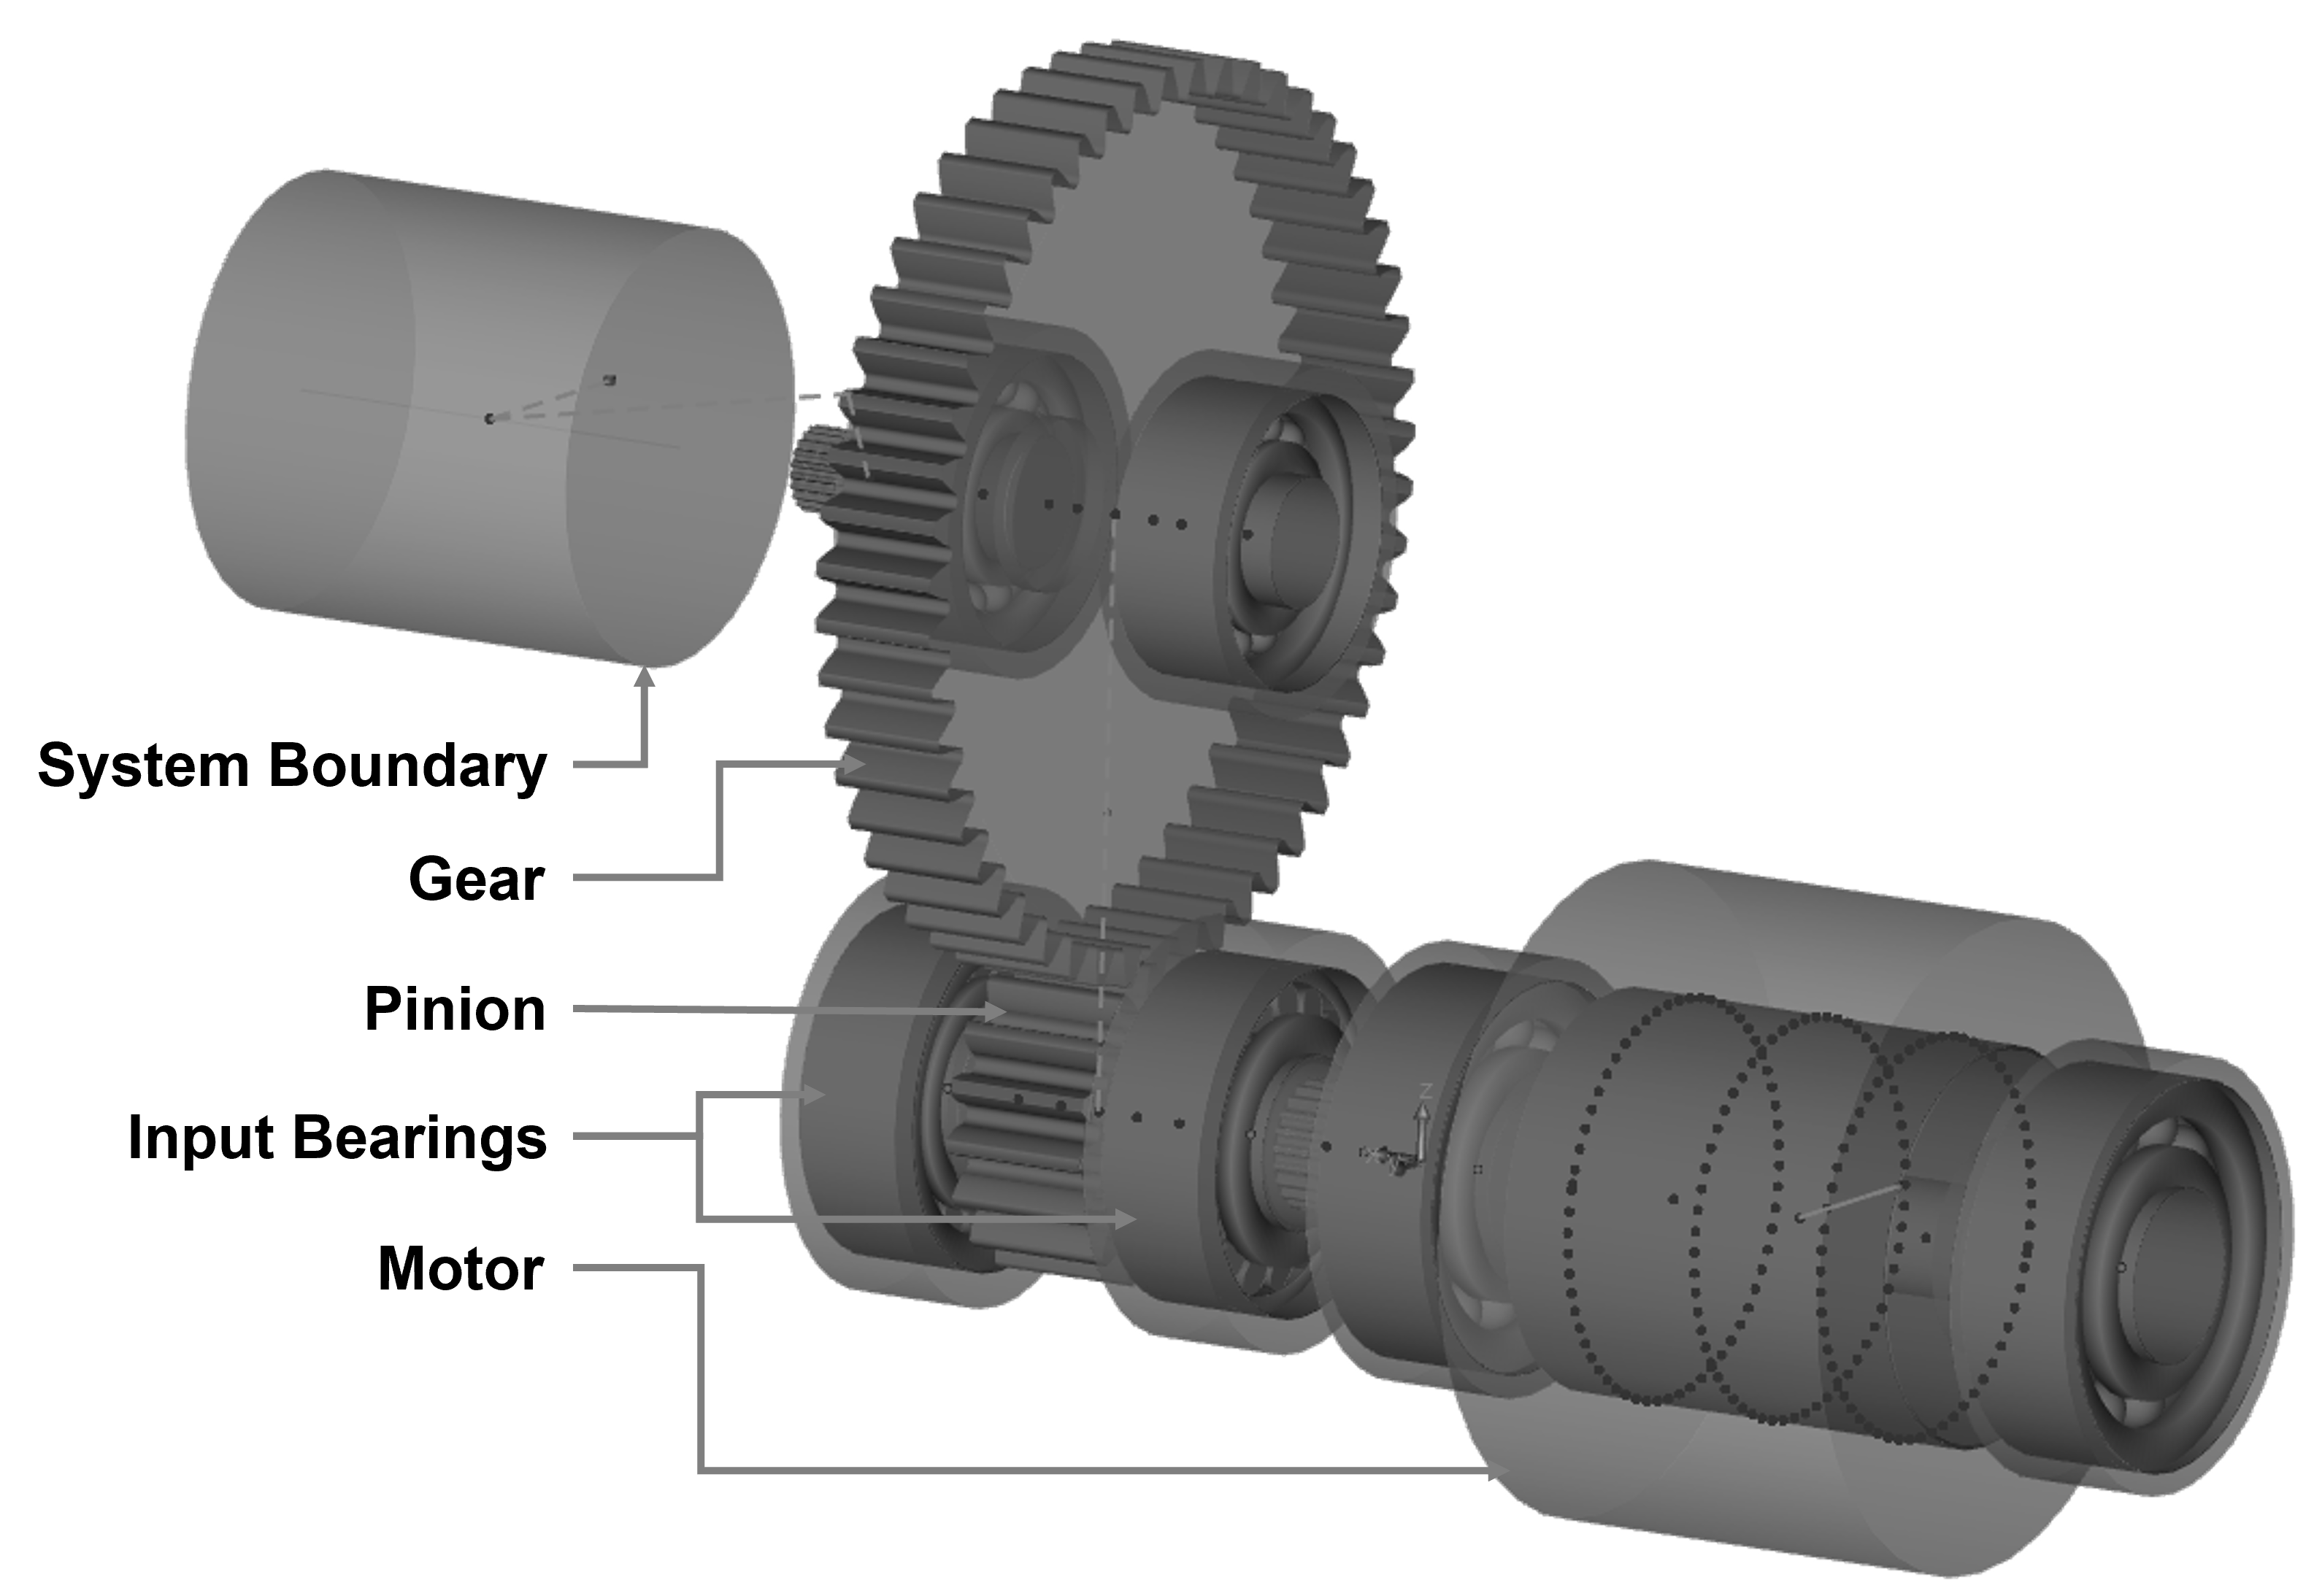
\includegraphics[width=125mm]{Hub_motor_excitation_model_annotated.png}
	\caption{Hub motor excitation model.}
	\label{Hub_motor_excitation_model}
\end{figure} 

\begin{table*}
	%\captionsetup{justification=centering}
	\caption{Pinion Geometry}
	\label{Pinion Geometry}
	\centering
	\renewcommand{\arraystretch}{1.5}%
	\begin{tabular}{|c|c|}
		\hline
		\ \textbf{Parameter} & \textbf{Value} \\ [0.5ex]
		\hline
		Number of teeth & 17 \\ [0.5ex]
		\hline
		Normal module & 0.004 $m$ \\ [0.5ex]
		\hline
		Normal pressure angle & 20 $^{\circ}$ \\ [0.5ex]
		\hline
		Helix angle at pitch circle & 0 $^{\circ}$ \\ [0.5ex]
		\hline
		Active tip diameter & 0.076 $m$ \\ [0.5ex]
		\hline
		Active root diameter & 0.065 $m$ \\ [0.5ex]
		\hline
		Width & 0.035 $m$ \\ [0.5ex]
		\hline
	\end{tabular}
\end{table*}

\begin{table*}
	%\captionsetup{justification=centering}
	\caption{Gear Geometry}
	\label{Gear Geometry}
	\centering
	\renewcommand{\arraystretch}{1.5}%
	\begin{tabular}{|c|c|}
		\hline
		\ \textbf{Parameter} & \textbf{Value} \\ [0.5ex]
		\hline
		Number of teeth & 51 \\ [0.5ex]
		\hline
		Normal module & 0.004 $m$ \\ [0.5ex]
		\hline
		Normal pressure angle & 20 $^{\circ}$ \\ [0.5ex]
		\hline
		Helix angle at pitch circle & 0 $^{\circ}$ \\ [0.5ex]
		\hline
		Active tip diameter & 0.212 $m$ \\ [0.5ex]
		\hline
		Active root diameter & 0.202 $m$ \\ [0.5ex]
		\hline
		Width & 0.030 $m$ \\ [0.5ex]
		\hline
	\end{tabular}
\end{table*}

\subsection{Co-Simulation of Coupled Models}
A coupled simulation approach is employed to implement the lubricated components level bearing model within the flexible multi-body dynamic (FMBD) environment. AVL EXCITE\textsuperscript{TM} Power Unit R2022.1 contains integrated “Link to MATLAB” functionality, whereby joints within the model can be replaced with a user function created in MATLAB Simulink\textregistered\ R2022b.

\paragraph{Connected Degrees of Freedom}

Connections are created between bodies in the FMBD software using pins. Pins are assigned to specific nodes on the shaft and housing. The pins transmit a 6-element vector that describe the 6 DOF of the connection point. The first 3 elements represent translational DOFs, whilst the latter represent rotational DOFs. This are concatenated into a single communication vector that is then transferred to MATLAB\textregistered\.

\begin{figure}
	\centering  
	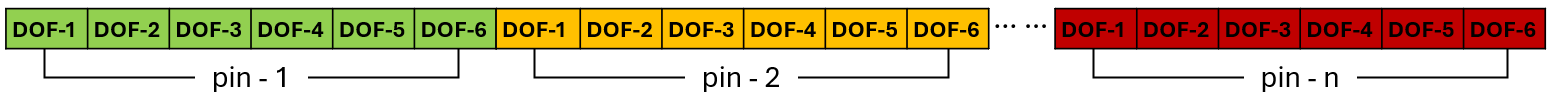
\includegraphics[width=150mm]{Communication_Vector_MATLAB.png}
	\caption{Communication vector and degrees of freedom.}
	\label{Communication_Vector_MATLAB}
\end{figure} 

Two vectors are transferred from EXCITE to MATLAB\textregistered\: one containing displacement information in all 6 DOF and the other containing velocity information. Force vectors of equal size are then computed within the component level model in MATLAB\textregistered\ and returned to EXCITE\textsuperscript{TM} Power Unit.

The connection to MATLAB\textregistered\ is facilitated via an S-function. Therefore, a Simulink\textregistered\ model is required. A generic block developed by AVL, the EXCITE\textsuperscript{TM} Power Unit Simulink\textregistered\ block, is used for this purpose:

\paragraph{Output Port}

Output data from the FMBD model is organised in vector format, of size 6$n$ where $n$ is the total number of connections being passed from MATLAB\textregistered\ to EXCITE\textsuperscript{TM} Power Unit. To access data for each connection, and then split this into specific DOFs, two levels of Demux elements are needed.

\begin{enumerate}
	\item The first level of Demux splits the output vector into $n$ pins, of size 6 to represent the DOFs at each pin. 
	\item The second level of Demux blocks splits the 6-element vector for each pin into the 6 scalar values that represent the data for each DOF. These can then be used as inputs to the MATLAB\textregistered\ function block within the Simulink\textregistered\ model.	
\end{enumerate}

\begin{figure}
	\centering  
	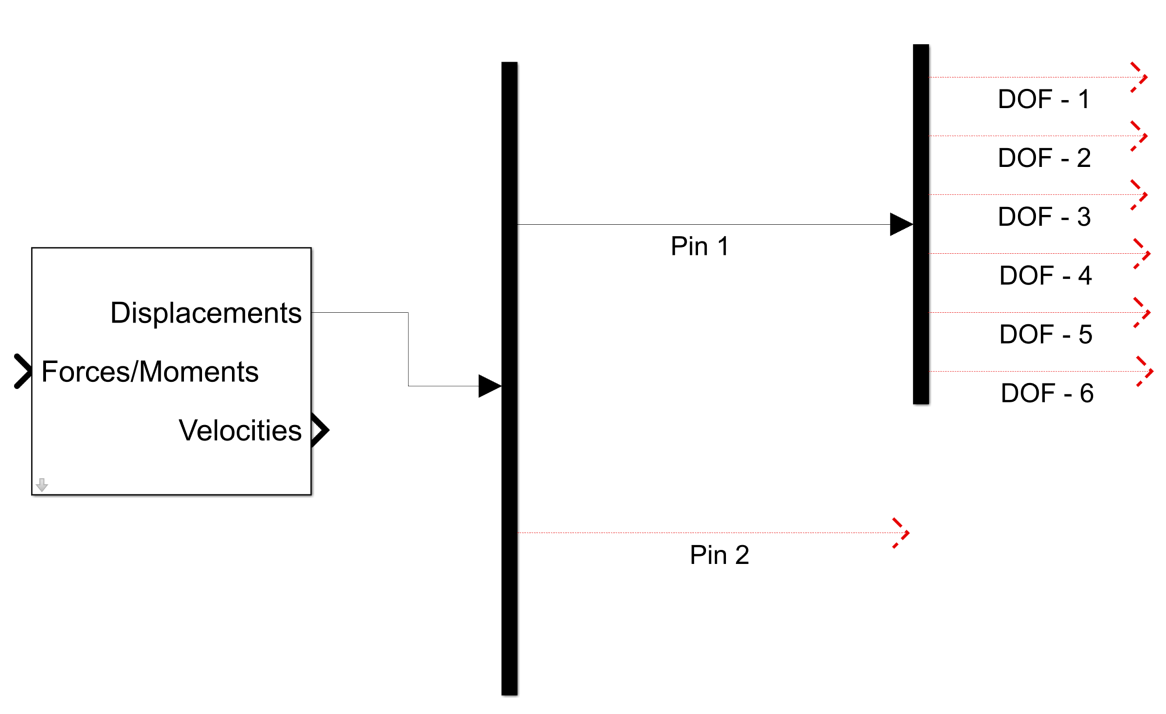
\includegraphics[width=125mm]{Output Port.png}
	\caption{Output port Demux blocks and degrees of freedom.}
	\label{Output Port Simulink}
\end{figure} 

\paragraph{Input Port}

At the input port to the EXCITE\textsuperscript{TM} Power Unit Simulink block, a vector of 6$n$ elements must be passed. This requires two Mux blocks: the first to combine the DOFs of each pin, and the second to combine all of these connection vectors into a single vector that is passed to EXCITE\textsuperscript{TM} Power Unit.

\begin{figure}
	\centering  
	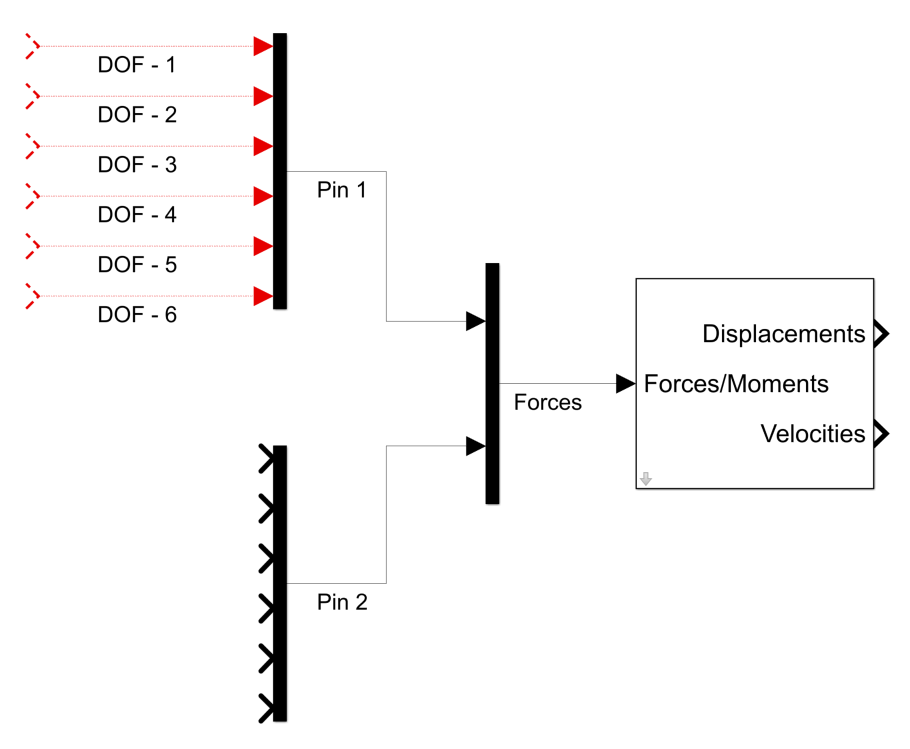
\includegraphics[width=125mm]{Input Port.png}
	\caption{Input port Mux blocks and degrees of freedom.}
	\label{Input Port Simulink}
\end{figure} 

\paragraph{Simulink Model}

To integrate the lubricated bearing model into the Simulink\textregistered\ model, the MATLAB\textregistered\ Function block is used. The input variable sizes are defined at the beginning of the function, and the appropriate DOFs are connected to the block in the order of which they appear in the function. The function blocks and hence lubricated bearing models are highlighted in \ref{Simulink_model_schematic}, as well as the ports and the demux blocks that split the DOFs.

\begin{figure}
	\centering  
	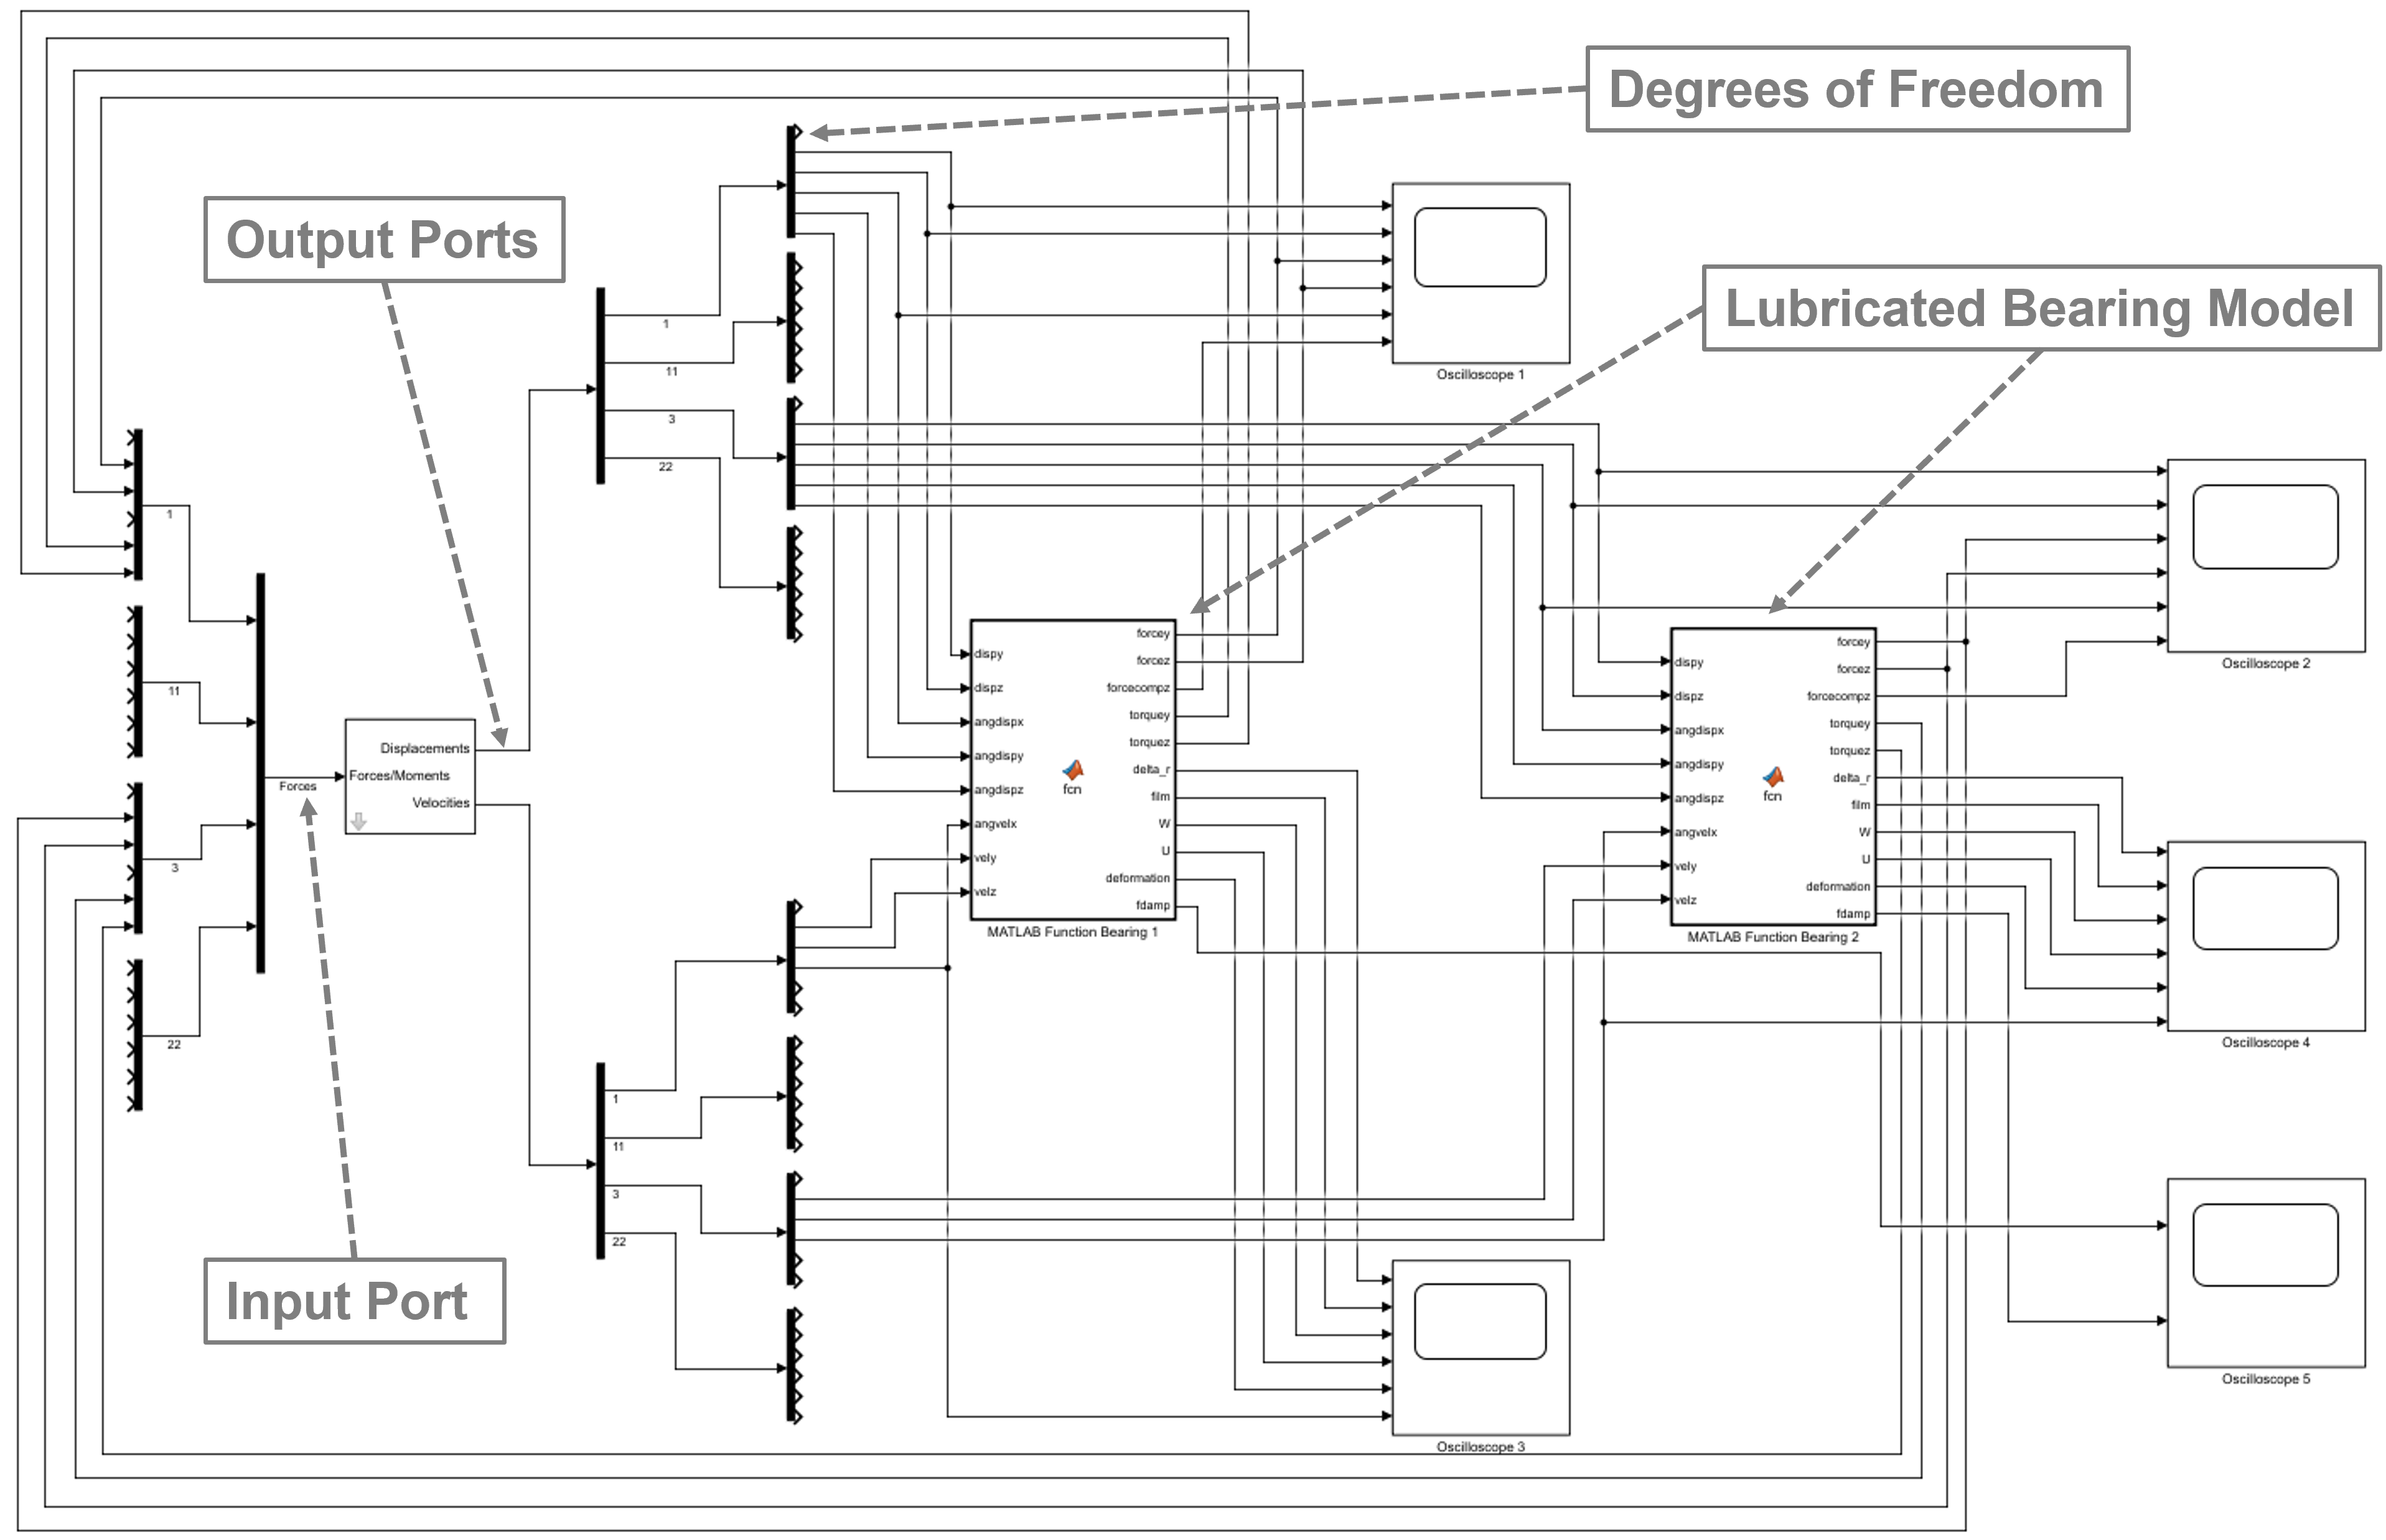
\includegraphics[width=150mm]{Simulink_schematic_annotated.png}
	\caption{Simulink\textregistered\ model schematic.}
	\label{Simulink_model_schematic}
\end{figure} 

The coupled simulation supported by EXCITE\textsuperscript{TM} Power Unit is explicit in nature. There is no iteration at each time step between the dynamic solver and the bearing model. Error accumulation can therefore lead to numerical divergence. Investigations were performed from 0.1~-~1$\times 10^{-5}$~$s$ in steps of 0.1~$\times 10^{-5}$~$s$. It was found that a simulation time step of 1$\times 10^{-6}$~$s$ was fine enough to ensure numerical convergence at all operating conditions, while also remaining computationally efficient.

\section{Results and Discussion}

A quasi-dynamic speed sweep has been performed from 1~000 to 21~000~$rpm$. The simulations are performed every 1000~$rpm$, refined to 250~$rpm$ intervals throughout a period of system resonance between 12~000~$rpm$ and 14~000~$rpm$. The operating envelopes are generated by plotting the maximum and minimum values from the steady-state signals at each speed interval. The conjunction level results are obtained from an individual roller and its contact with the inner raceway. The component and system level results are taken from the geometric centre of the inner bearing race, corresponding to the bearing seat on the shaft. The following figures represent results in the $y$-direction, the largest component of excitation due to the tangential force from the gear meshing.

The contact level results (Figure \ref{Rolling element contact stiffness - Dry vs lubricated maximum values}) show a difference in the contact stiffness between the dry and lubricated models. The dry model follows the torque profile of the motor, with stiffness decreasing as the contact forces reduce. The period of resonance leads to the larger amplitude excitation of the shaft, resulting in an increase in the contact stiffness due to the force–deflection non-linearity. The lubricated model, however, shows an increase in the contact stiffness throughout the speed sweep. This is due to the higher levels of deformation at the contact as the lubricant is entrained, which increases with the shaft rotational velocity. This behaviour was experimentally observed by Dietl, concluding that the oil-wedge between the rolling elements and raceways reduces the internal clearance of the bearing and increases its stiffness \cite{Dietl1997}. The contact stiffness in the lubricated bearing model under the same operating conditions is therefore 24.9\% greater at 21~000~$rpm$.

\begin{figure}
	\centering  
	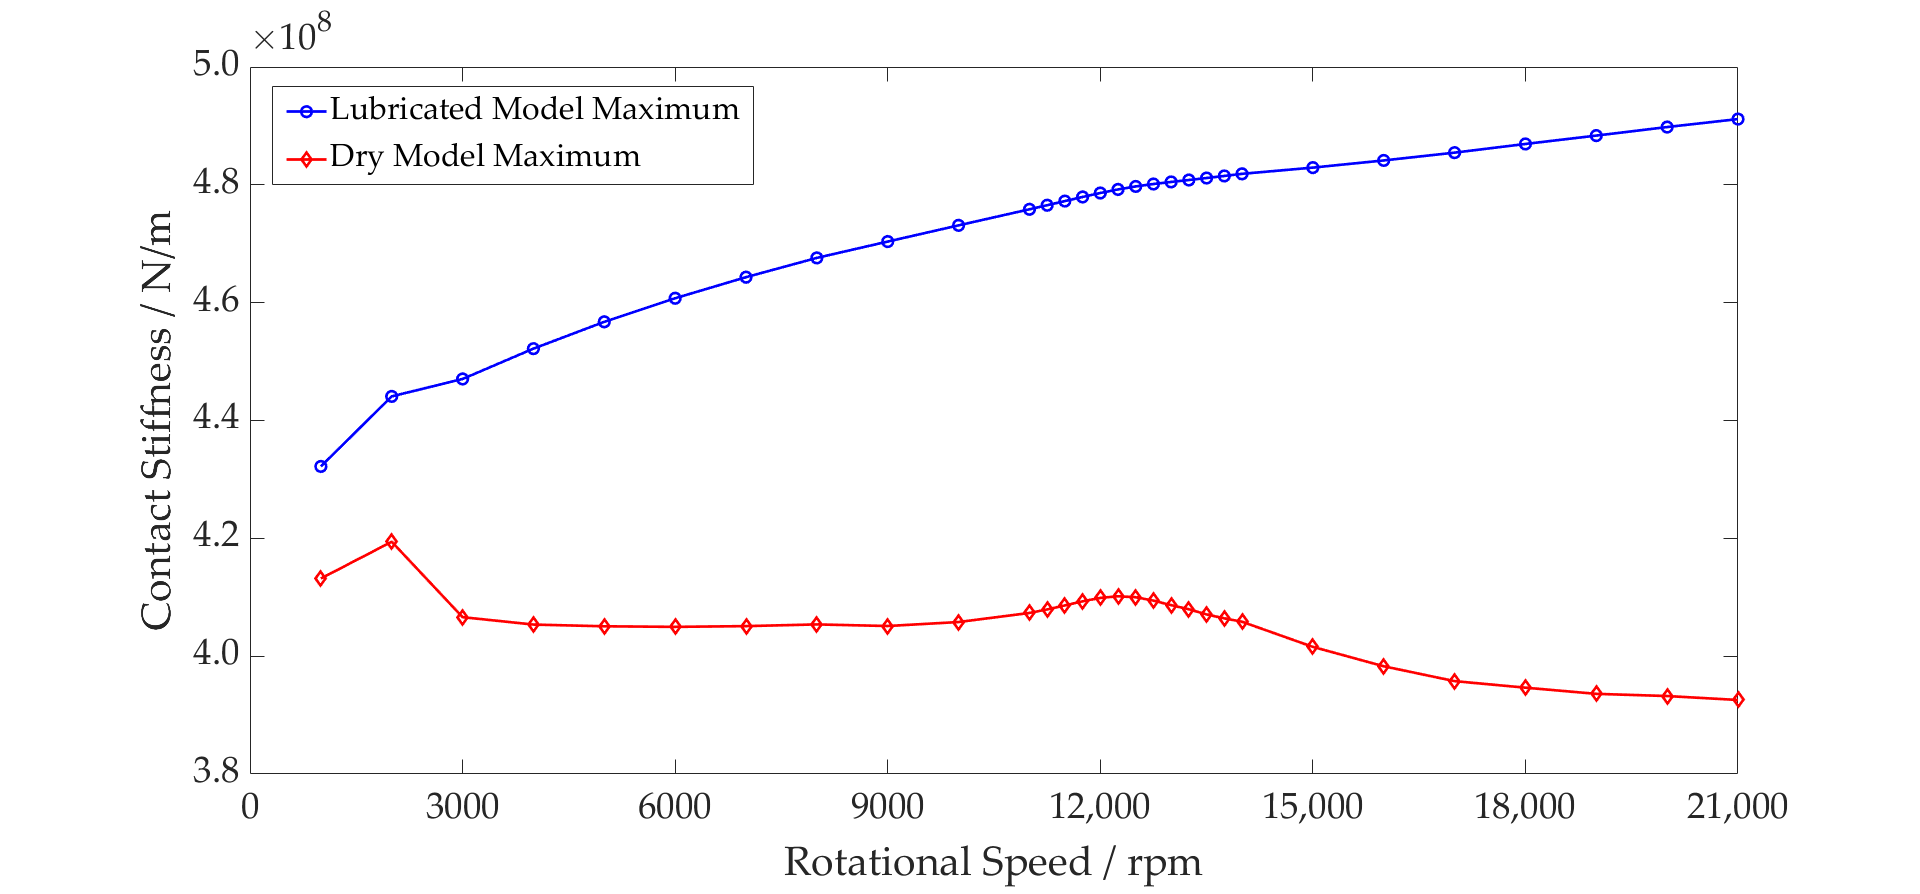
\includegraphics[width=150mm]{FlexiTribo Figure 7. Rolling Element Contact Stiffness - Dry vs Lubricated Maximum Values.png}
	\caption{Rolling element contact stiffness - Dry vs lubricated maximum values.}
	\label{Rolling element contact stiffness - Dry vs lubricated maximum values}
\end{figure} 

The peak contact force has been compared between both models. The percentage increase between the dry and lubricated models is shown in Figure \ref{Rolling element contact force - Dry vs lubricated percentage increase}. This more clearly shows the disparity between both models at the contact, with the largest difference being 9.6 times at maximum speed. During resonance, the inner race force reaches a peak of 1~514~$\mathrm{N}$, resulting in surface deformation magnitudes of 0.92~$\mu \mathrm{m}$ and 3.81~$\mu \mathrm{m}$ at the dry and lubricated conjunctions, respectively. As noted in previous works [15], higher loads lead to a greater surface deformation to the film thickness ratio, causing the percentage difference between the dry and lubricated models to reduce. Once the loads reduce as the speed increases, the percentage increase continues to rise.

\begin{figure}
	\centering  
	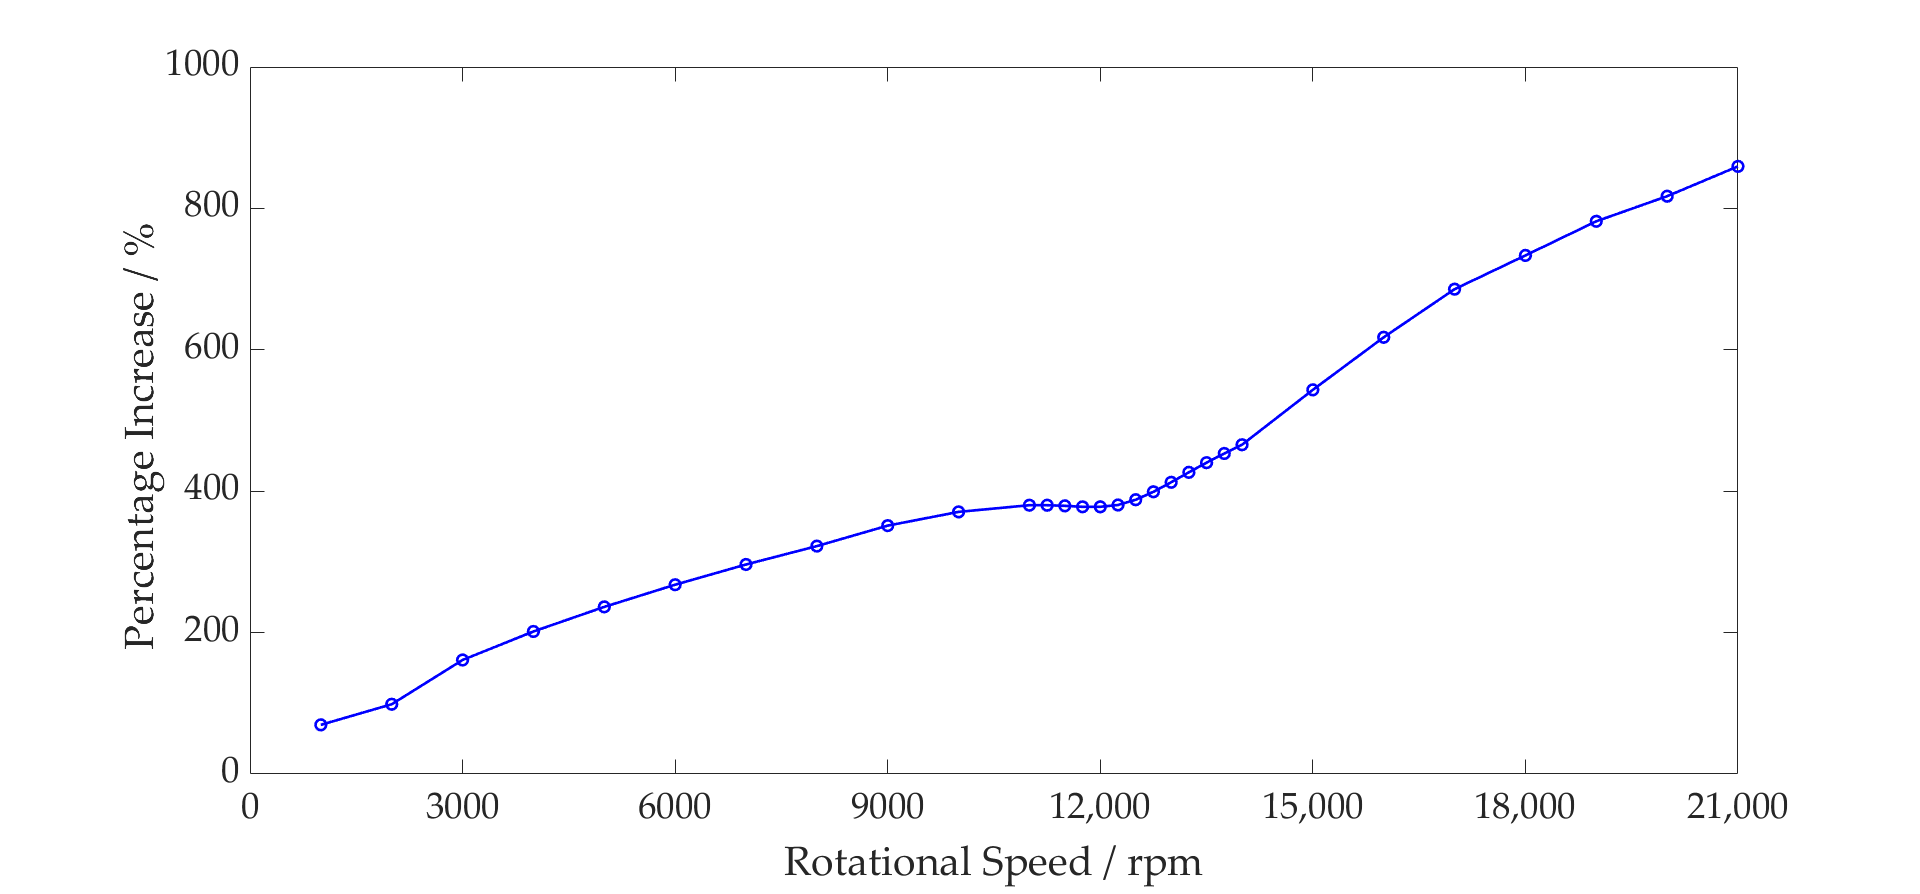
\includegraphics[width=150mm]{FlexiTribo Figure 8. Rolling Element Contact Force - Dry vs Lubricated Percentage Increase.png}
	\caption{Rolling element contact force - Dry vs lubricated percentage increase.}
	\label{Rolling element contact force - Dry vs lubricated percentage increase}
\end{figure} 

The total bearing stiffness is a combination of all contact stiffnesses between the elements and raceways. These contact stiffnesses vary non-linearly with force, resulting in the total bearing stiffness varying accordingly. For the dry model, this is clearly demonstrated, with the greater total bearing stiffness at the peak of the resonance due to the greater bearing forces (see Figure \ref{Inner race stiffness - Dry vs lubricated operating envelope}). This does not, however, capture the change of the total bearing stiffness with speed; the average bearing stiffness does not change. The lubricated bearing is not only stiffer than the dry bearing, but this stiffness also increases with speed. This is shown in Figure \ref{Inner race stiffness - Dry vs lubricated operating envelope} by the non-linear increase in the average lubricated bearing stiffness values compared to the constant values for the dry model. The combination of these two factors leads to the lubricated model having a $16.6 \%$ greater maximum total bearing stiffness at 21~000~$\mathrm{rpm}$ than the dry model.

\begin{figure}
	\centering  
	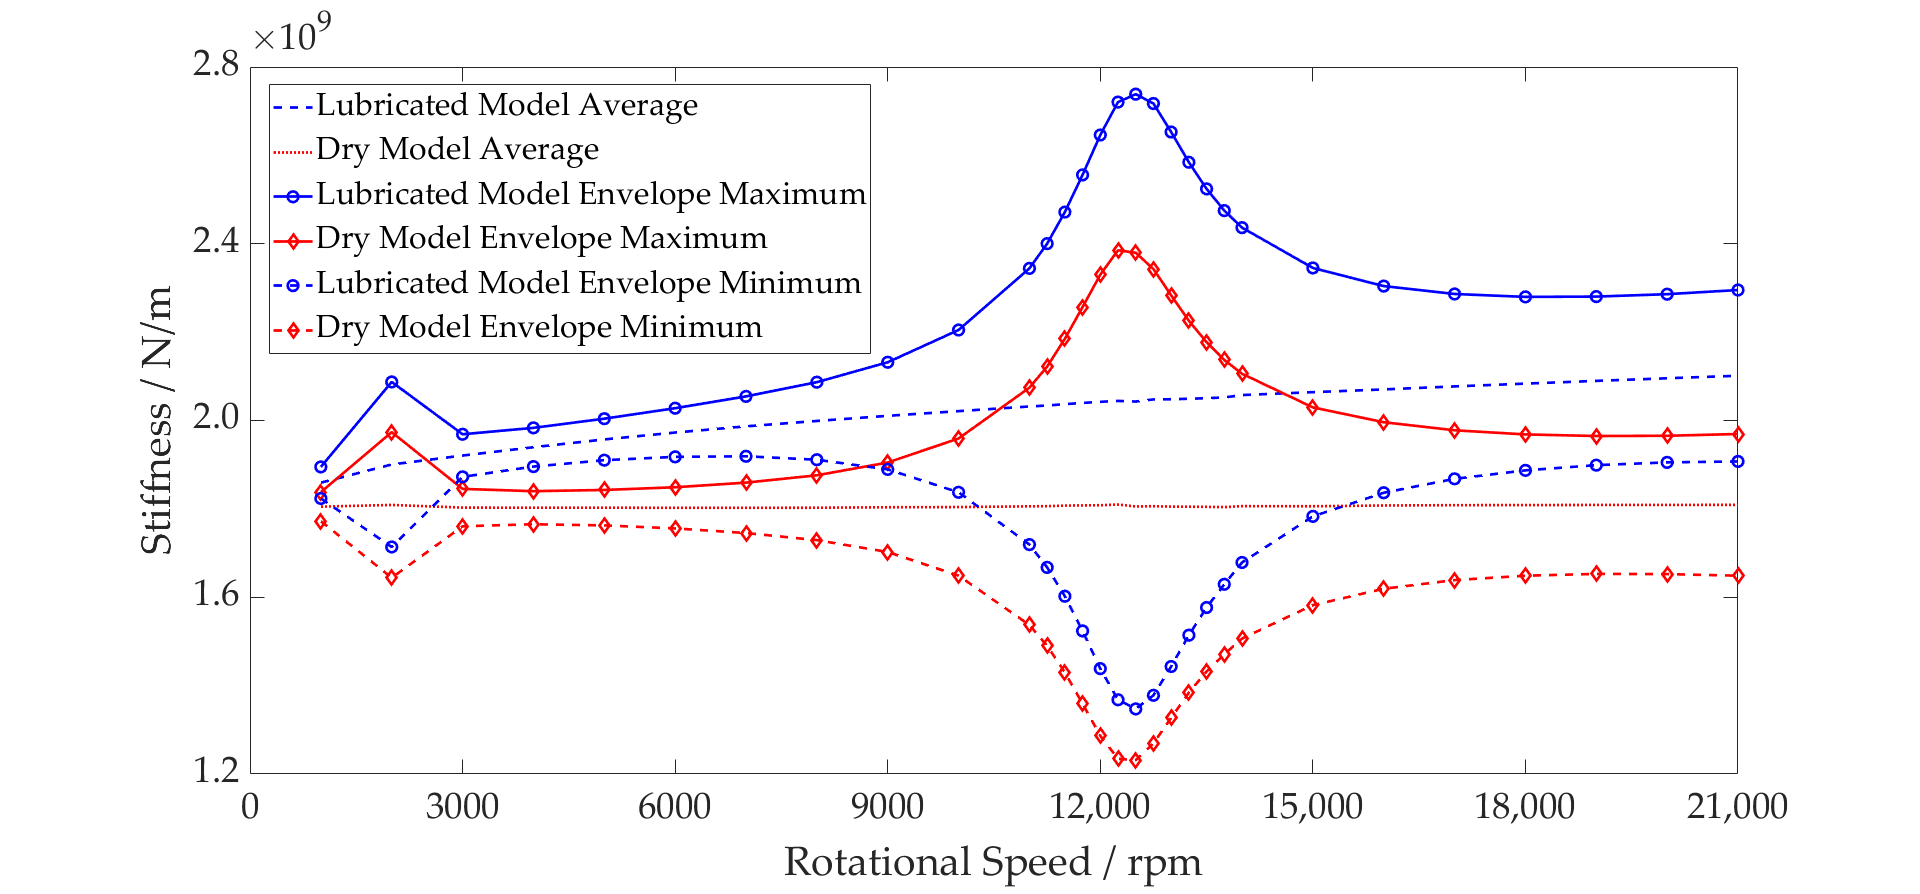
\includegraphics[width=150mm]{FlexiTribo Figure 9. Inner Race Stiffness - Dry vs Lubricated Operating Envelope.png}
	\caption{Inner race stiffness - Dry vs lubricated operating envelope.}
	\label{Inner race stiffness - Dry vs lubricated operating envelope}
\end{figure} 

Due to the greater total stiffness of the bearing, the shaft displacement of the lubricated model is lower both on average and peak to peak for the same applied force in comparison to the dry model (see Figure \ref{Inner race displacement - Dry vs lubricated operating envelope}). Through the period of resonance, the large inner race forces result in the roller–race separation of the unloaded rollers within the dry model. This leads to greater shaft displacement as the inner race moves into this region of zero stiffness until roller–race contact is made, and a reaction force is established.

\begin{figure}
	\centering  
	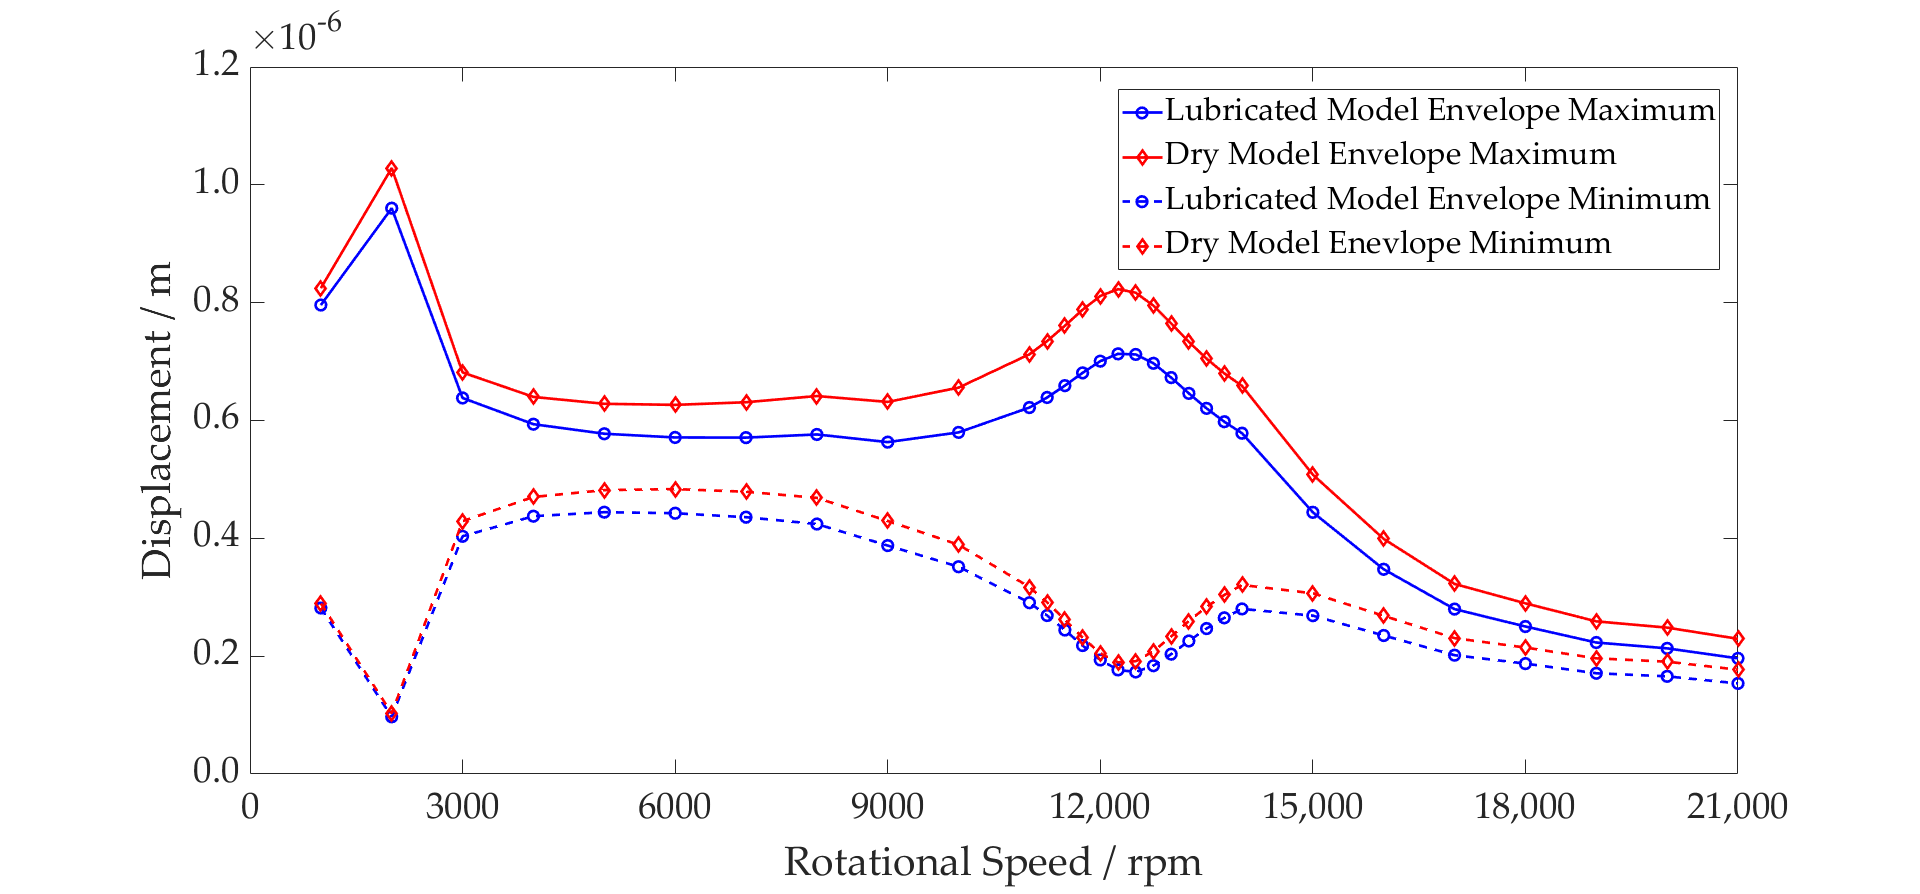
\includegraphics[width=150mm]{FlexiTribo Figure 10. Inner Race Displacement - Dry vs Lubricated Operating Envelope.png}
	\caption{Inner race displacement - Dry vs lubricated operating envelope.}
	\label{Inner race displacement - Dry vs lubricated operating envelope}
\end{figure} 

Figure \ref{Inner race acceleration - Dry vs lubricated operating envelope} shows that the acceleration peak of the system resonance occurs at 12~500~$\mathrm{rpm}$ (3~5420$\mathrm{Hz}$) for the lubricated model as opposed to 12~250~$\mathrm{rpm}$ (3~470~$\mathrm{Hz}$) for the dry model. This shift in natural frequency indicates a stiffer overall system. The magnitude difference between the dry and lubricated models can also be attributed to the unloaded regions of the dry bearing. The contact deformation arising from the loading of the inner race is sufficient to cause the rollers geometrically opposite to become separated from their contacts. Contact is lost between the roller and raceway, leading to zero contact stiffness. The inner race moves into this region until it is reacted by a contact force once again. These regions of zero stiffness are shown in Figure \ref{Rolling element contact stiffness - Dry vs lubricated minimum values}, where the minimum stiffness of an individual rolling element and raceway contact in the dry model drops to zero due to separation. For the lubricated model, contact is maintained throughout.

\begin{figure}
	\centering  
	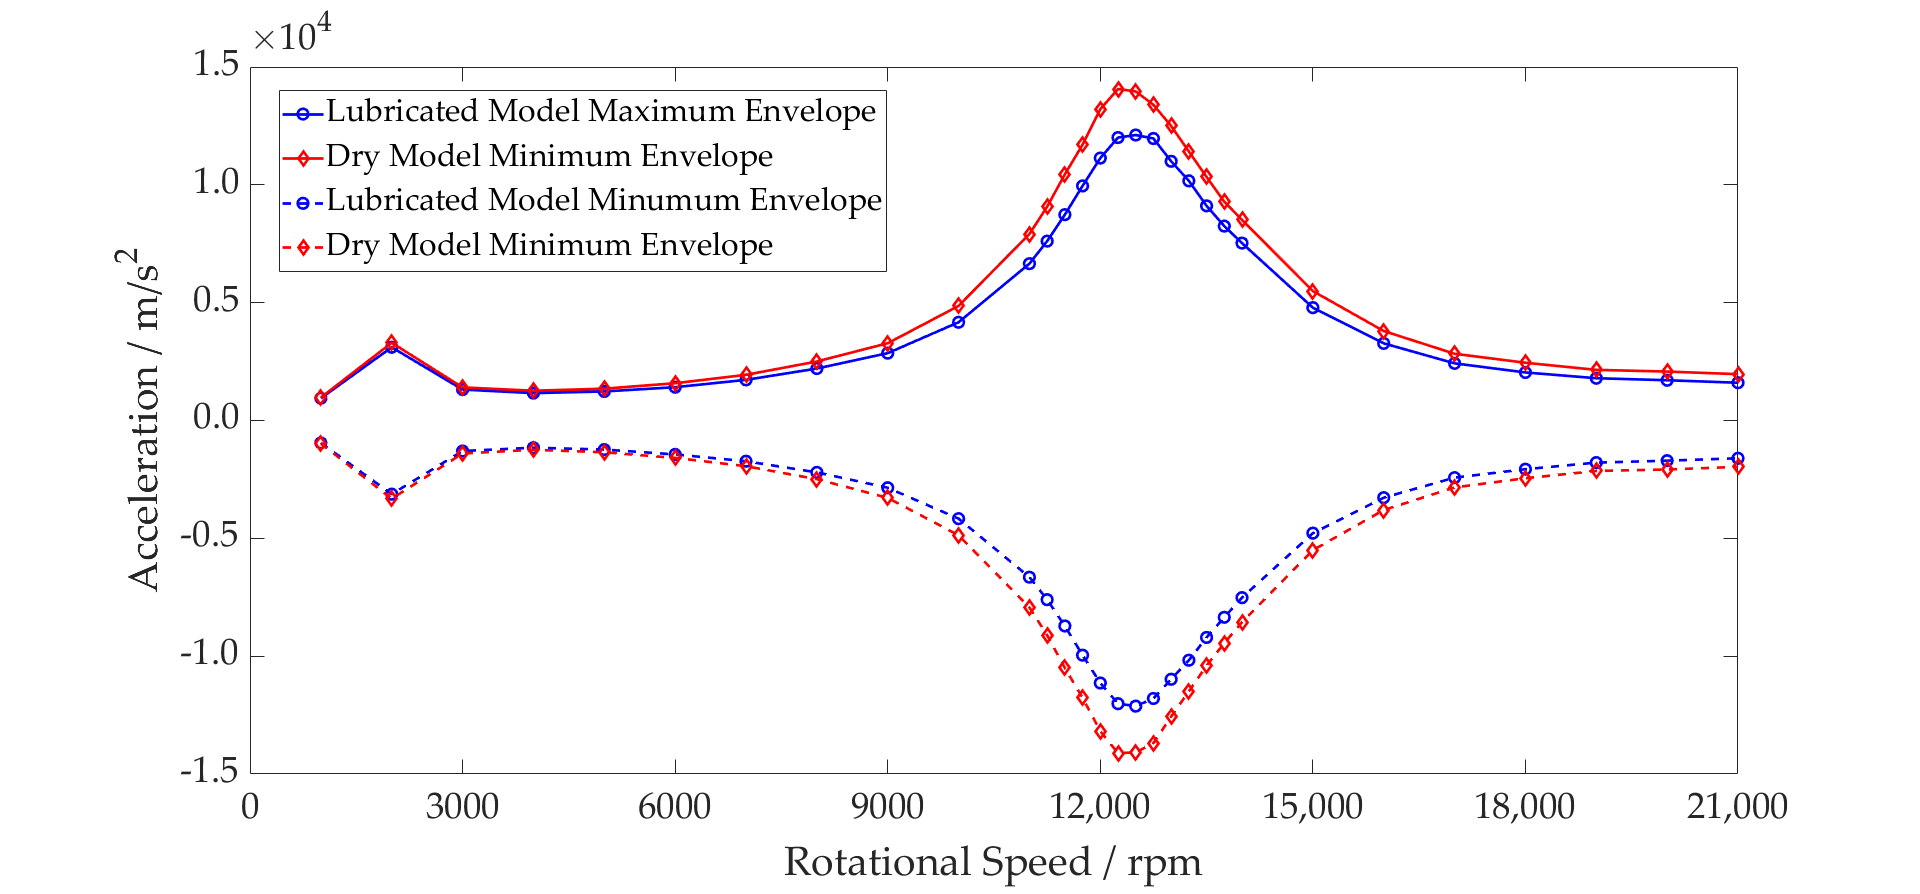
\includegraphics[width=150mm]{FlexiTribo Figure 11. Inner Race Acceleration - Dry vs Lubricated Operating Envelope.png}
	\caption{Inner race acceleration - Dry vs lubricated operating envelope.}
	\label{Inner race acceleration - Dry vs lubricated operating envelope}
\end{figure}

\begin{figure}
	\centering  
	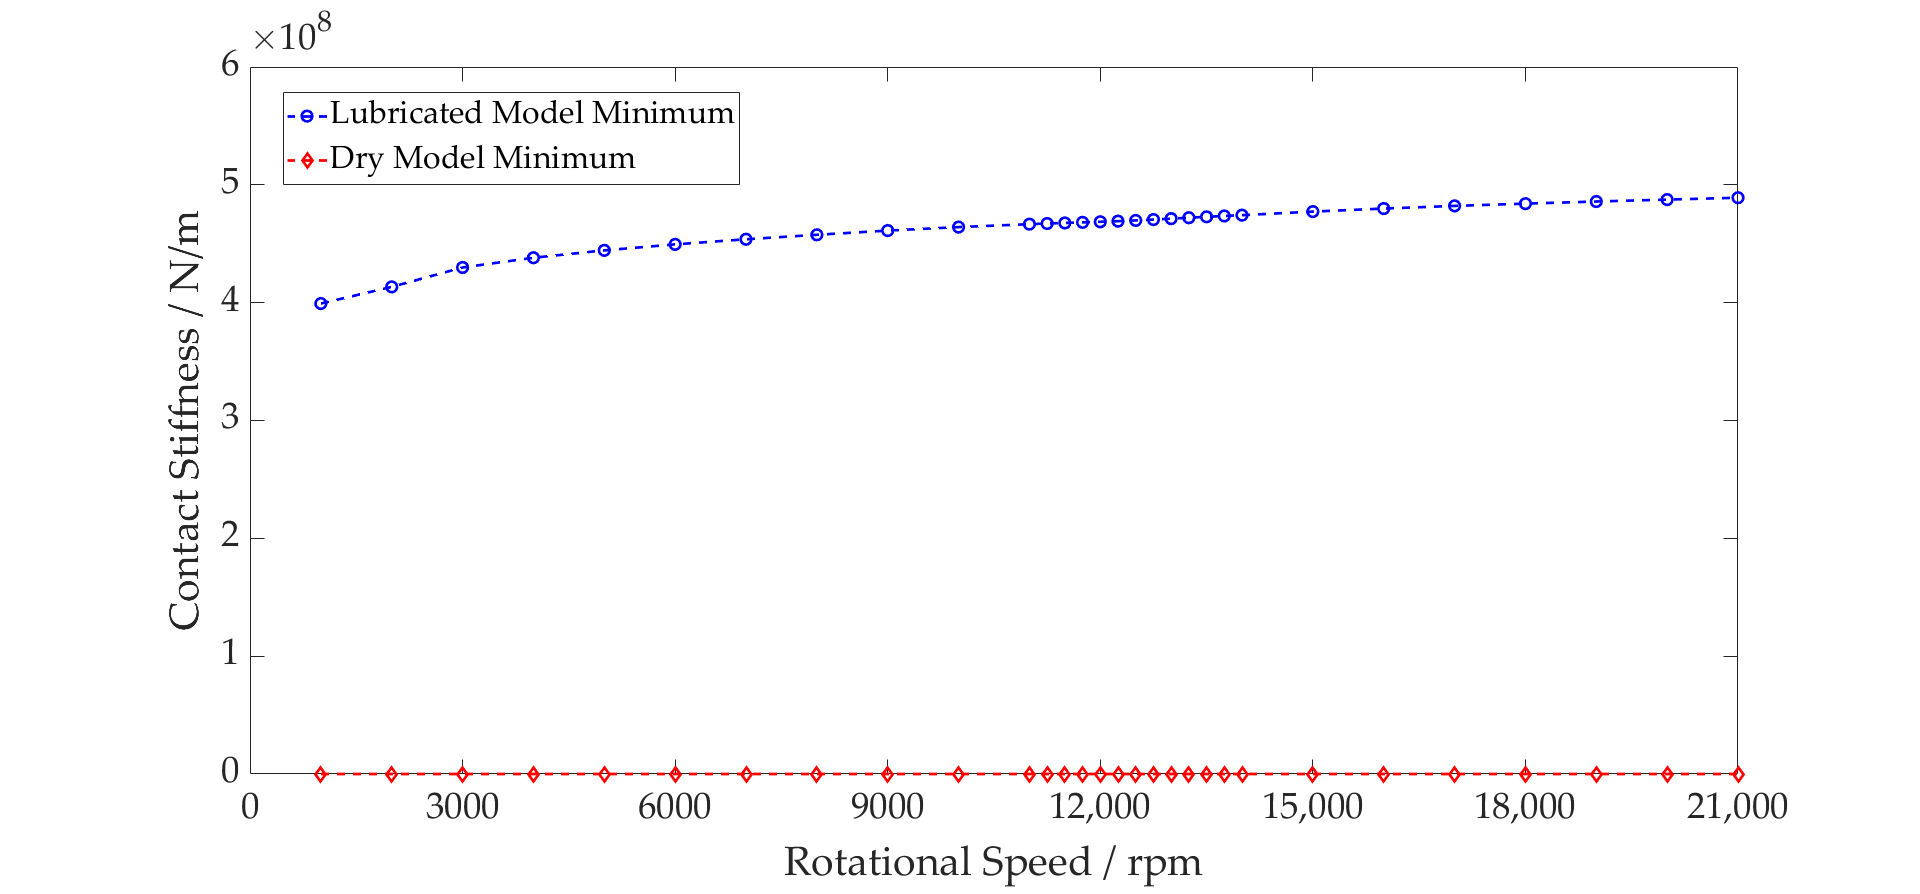
\includegraphics[width=150mm]{FlexiTribo Figure 12. Rolling Element Contact Stiffness - Dry vs Lubricated Minimum Values.png}
	\caption{Rolling element contact stiffness - Dry vs lubricated minimum values.}
	\label{Rolling element contact stiffness - Dry vs lubricated minimum values}
\end{figure}

Analysing the conjunction level results from the lubricated model, the contact force due to the gear mesh frequency is shown superimposed on the ball pass frequency as an individual element passes through the loaded region of the bearings (Figures \ref{Film thickness vs contact force 21 000 rpm} and \ref{Film thickness vs contact force 12 500 rpm}). The higher contact forces result in a reduction in the central film thickness, also shown when observing the variation in film thickness for both plots. At 12~500~$\mathrm{rpm}$, the force and film thickness fluctuations are much larger due to the high excitation levels of the shaft during resonance. At 21~000~$\mathrm{rpm}$, even with a much lower torque transfer through the gear pair, the contact forces are greater than at 12~500~$\mathrm{rpm}$. This is due to the contribution of the film enhancing the total contact deflection and hence increasing the contact force.

\begin{figure}
	\centering  
	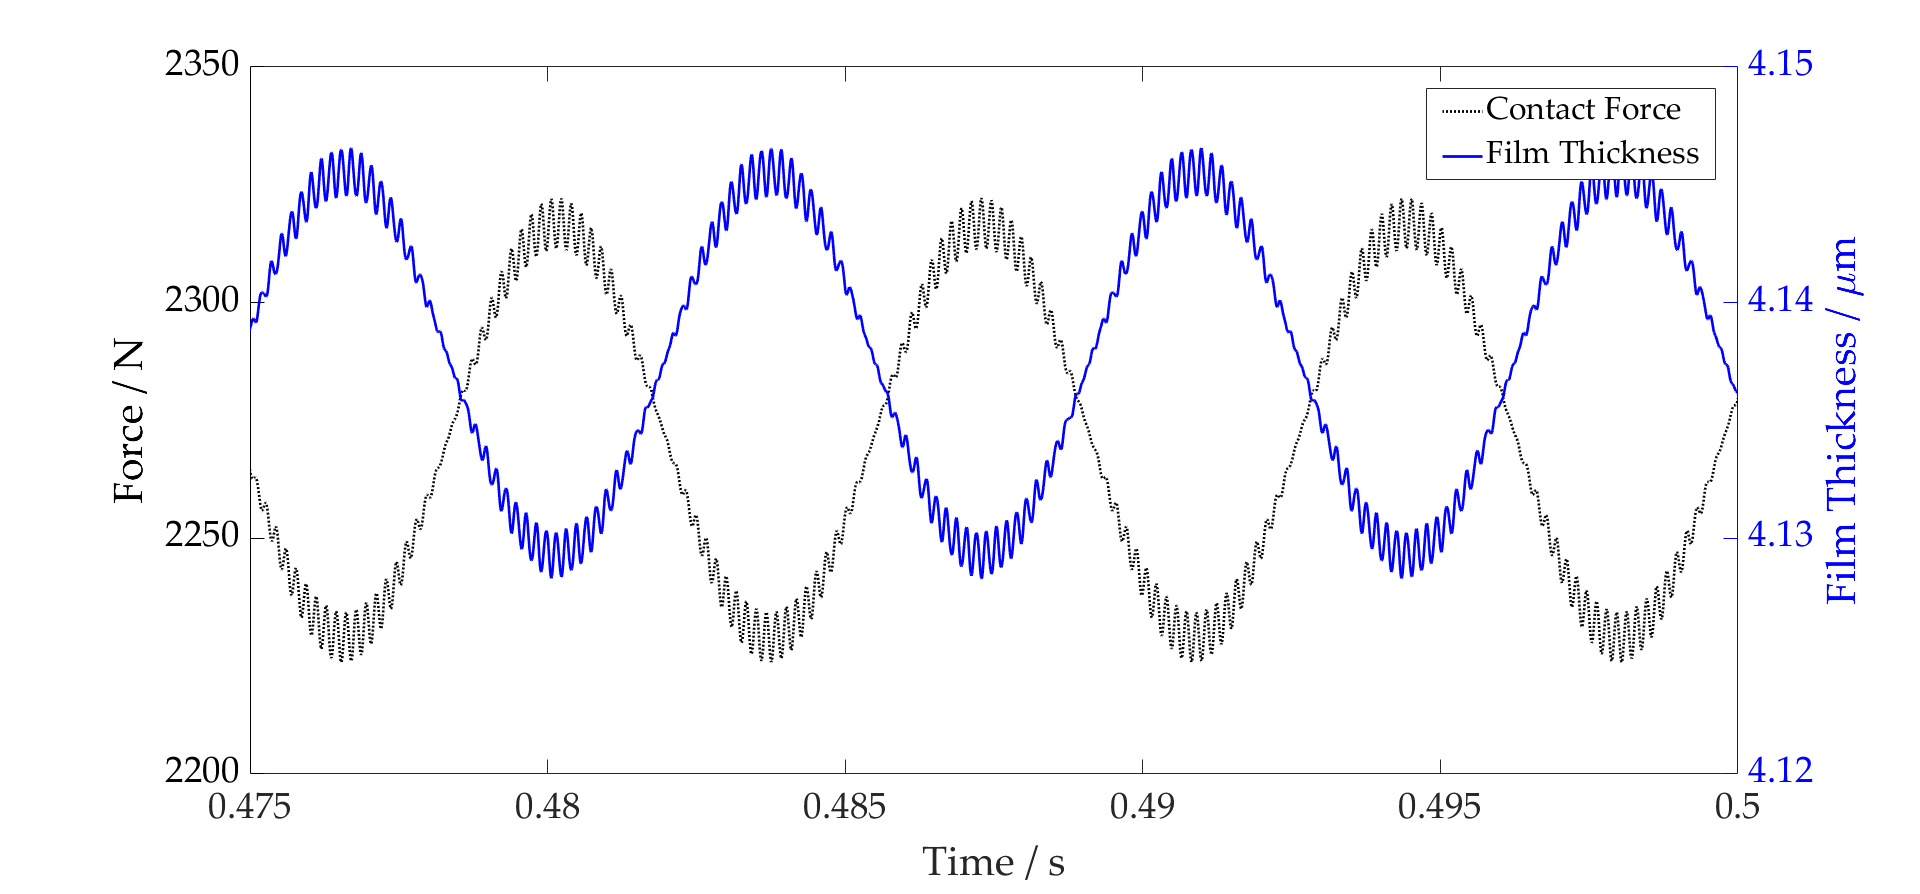
\includegraphics[width=150mm]{FlexiTribo Figure 13. Film Thickness vs Contact Force 21 000 rpm.png}
	\caption{Film thickness vs contact force 21~000~$\mathrm{rpm}$.}
	\label{Film thickness vs contact force 21 000 rpm}
\end{figure}

\begin{figure}
	\centering  
	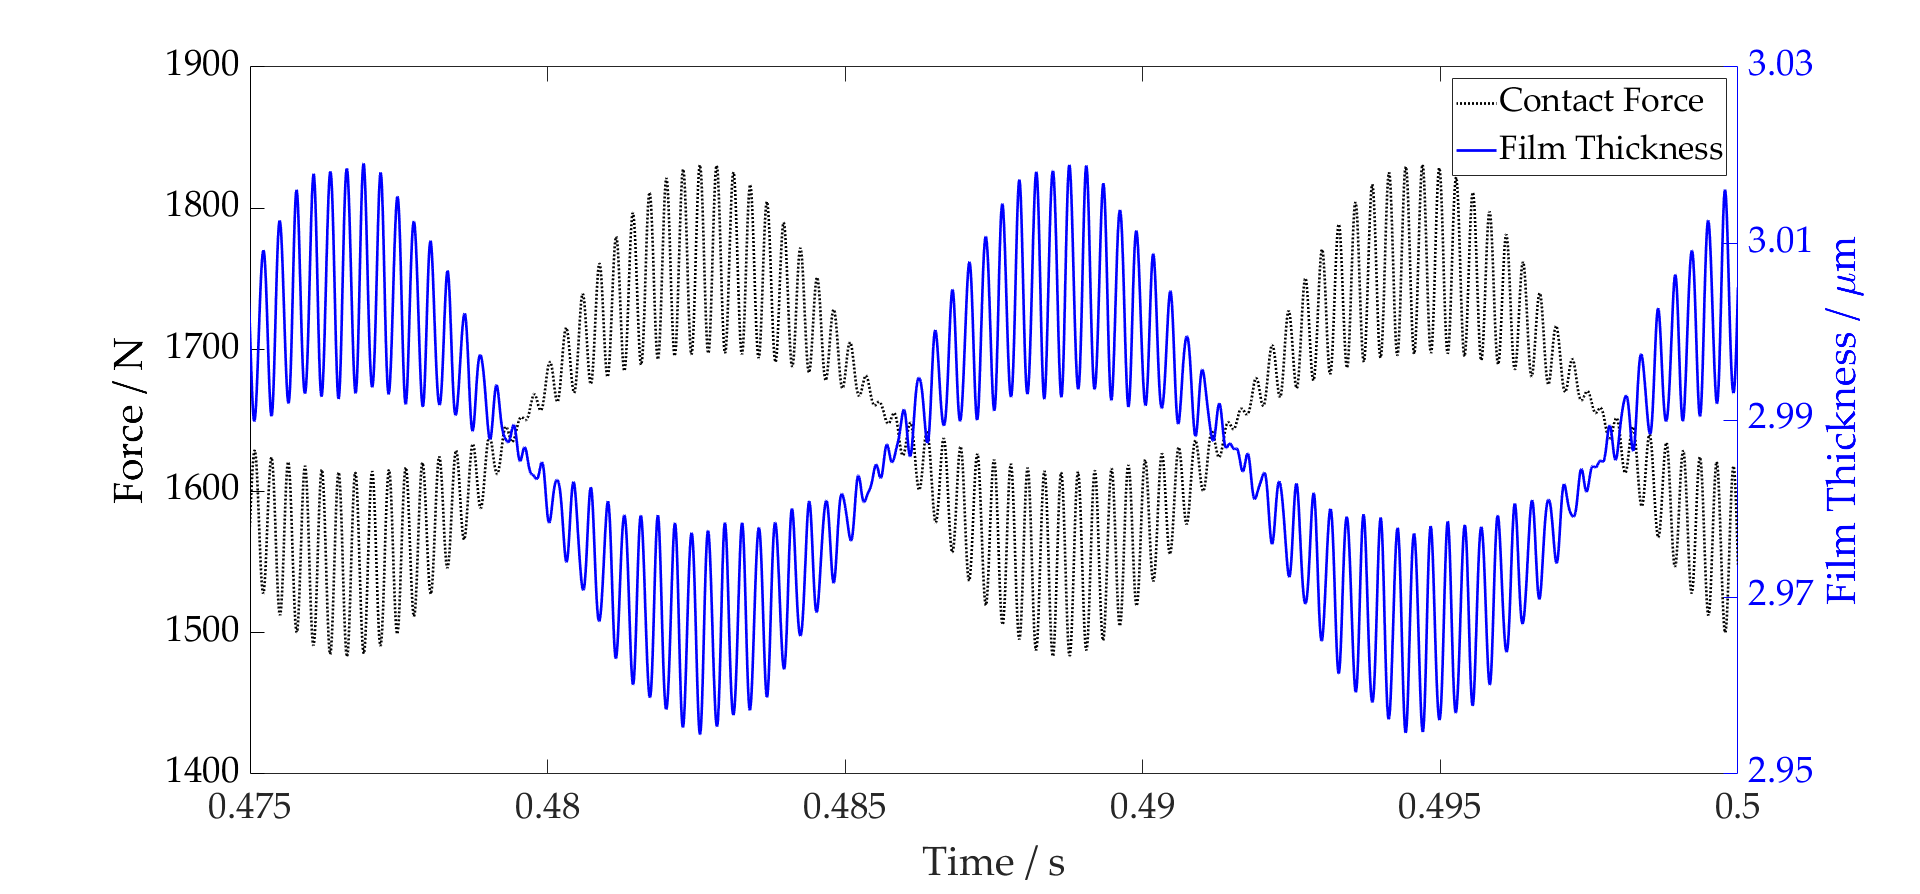
\includegraphics[width=150mm]{FlexiTribo Figure 14. Film Thickness vs Contact Force 12 500 rpm.png}
	\caption{Film thickness vs contact force 12~500~$\mathrm{rpm}$.}
	\label{Film thickness vs contact force 12 500 rpm}
\end{figure}

\subsection{Conclusions}

The new methodology presented has been developed to implement a lubricated bearing model within a flexible system level model. The following conclusions are drawn:

\begin{enumerate} 
	\item Simulations have been performed up to 21~000~$\mathrm{rpm}$ with realistic excitation forces from a first stage reduction gear pair and electric motor. The FMBD model implicitly includes the lubricant film at the roller–race contact within the bearing; The conjunction level and system level results have been analysed to compare the lubricated and conventional dry-bearing modelling techniques. This is something that has not, to the authors’ knowledge, been reported previously in the open literature.
	\item Results show that the film thickness reaches 4.15~${\mu m}$ at 21~000~$\mathrm{rpm}$. This leads to 9.6 times greater contact forces and hence 24.9\% greater contact stiffness between the dry and lubricated models due to the lubricant entrainment and non-linear Hertzian force–deflection relationship. 
	\item The contribution of all the rolling elements leads to the lubricated model having a 16.6\% greater maximum total bearing stiffness at 21~000~$\mathrm{rpm}$ than the dry model. Moreover, this stiffness is shown to increase with speed due to the film thickness increasing with the entrainment velocity; this is something that dry models do not account for.
	\item This increase in the total bearing stiffness leads to a change in the stiffness of the total system. By modelling the shaft as a flexible body, the influence on the natural frequency of the system is seen. The resonant peak at 12~500~$\mathrm{rpm}$ shifts 250~$\mathrm{rpm}$ higher in the lubricated model, which coincides with the higher frequency excitation from the gear meshing.
\end{enumerate}

Understanding the influence of the roller bearings on the transmission stiffness is of particular importance in automotive applications, and this change shows the effect of the lubricant film on the already complex contact phenomena. Neglecting the effect of the lubricant film can lead to an underestimation of the bearing stiffness, impacting the accuracy of dynamic analyses such as noise, vibration and harshness (NVH) prediction. 

As transmissions operate at higher speeds with more complex interconnected structures and noise paths, it is important that these behaviours are modelled accurately. Furthermore, underestimation of the contact forces will also lead to a miscalculation of contact pressures, impacting future sub-surface stress and wear analyses for the life predictions of these crucial critical  machine elements.



